\documentclass{sigchi}

% Use this command to override the default ACM copyright statement
% (e.g. for preprints).  Consult the conference website for the
% camera-ready copyright statement.


%% EXAMPLE BEGIN -- HOW TO OVERRIDE THE DEFAULT COPYRIGHT STRIP -- (July 22, 2013 - Paul Baumann)
% \toappear{Permission to make digital or hard copies of all or part of this work for personal or classroom use is      granted without fee provided that copies are not made or distributed for profit or commercial advantage and that copies bear this notice and the full citation on the first page. Copyrights for components of this work owned by others than ACM must be honored. Abstracting with credit is permitted. To copy otherwise, or republish, to post on servers or to redistribute to lists, requires prior specific permission and/or a fee. Request permissions from permissions@acm.org. \\
% {\emph{CHI'14}}, April 26--May 1, 2014, Toronto, Canada. \\
% Copyright \copyright~2014 ACM ISBN/14/04...\$15.00. \\
% DOI string from ACM form confirmation}
%% EXAMPLE END -- HOW TO OVERRIDE THE DEFAULT COPYRIGHT STRIP -- (July 22, 2013 - Paul Baumann)


% Arabic page numbers for submission.  Remove this line to eliminate
% page numbers for the camera ready copy 

%\pagenumbering{arabic}

% Load basic packages
\usepackage{balance}  % to better equalize the last page
\usepackage{graphics} % for EPS, load graphicx instead 
%\usepackage[T1]{fontenc}
\usepackage{txfonts}
\usepackage{times}    % comment if you want LaTeX's default font
\usepackage[pdftex]{hyperref}
% \usepackage{url}      % llt: nicely formatted URLs
\usepackage{color}
\usepackage{textcomp}
\usepackage{booktabs}
\usepackage{ccicons}
\usepackage{todonotes}
\usepackage{subfigure}
\usepackage{multirow}

% llt: Define a global style for URLs, rather that the default one
\makeatletter
\def\url@leostyle{%
  \@ifundefined{selectfont}{\def\UrlFont{\sf}}{\def\UrlFont{\small\bf\ttfamily}}}
\makeatother
\urlstyle{leo}

% To make various LaTeX processors do the right thing with page size.
\def\pprw{8.5in}
\def\pprh{11in}
\special{papersize=\pprw,\pprh}
\setlength{\paperwidth}{\pprw}
\setlength{\paperheight}{\pprh}
\setlength{\pdfpagewidth}{\pprw}
\setlength{\pdfpageheight}{\pprh}

% Make sure hyperref comes last of your loaded packages, to give it a
% fighting chance of not being over-written, since its job is to
% redefine many LaTeX commands.
\definecolor{linkColor}{RGB}{6,125,233}
\hypersetup{%
  pdftitle={SIGCHI Conference Proceedings Format},
  pdfauthor={LaTeX},
  pdfkeywords={SIGCHI, proceedings, archival format},
  bookmarksnumbered,
  pdfstartview={FitH},
  colorlinks,
  citecolor=black,
  filecolor=black,
  linkcolor=black,
  urlcolor=linkColor,
  breaklinks=true,
}

% create a shortcut to typeset table headings
% \newcommand\tabhead[1]{\small\textbf{#1}}

% End of preamble. Here it comes the document.
\begin{document}
\author{
  Yvonne Chen\\
  \texttt{evechen@uw.edu}
  \and
  Eleanor O'Rourke\\
  \texttt{eorourke@cs.washington.edu}
}
\title{Visualizing Student Problem-Solving Data}


\maketitle

\begin{abstract}
Much work in the education field highlights the importance of exposing student data to teachers, who can use it to provide students with timely and accurate assistance. However, there is little research that shows how best to visualize such data. The Enlearn tablet-based math curriculum software displays two visualizations, but they do not present data in a way that matches teacher needs. Building upon these visualizations, we create a system that demonstrates two new visual encodings of real-time student data. Informal feedback on our system is positive, and we aim to pilot our visualizations with teachers in an actual classroom setting.
\end{abstract}


%\keywords{Technology in the classroom; tablets for education; adaptive learning environments.}

%\category{H.5.0.}{Information Interfaces and Presentation}{General}

\section{Introduction}
%An explanation of the problem and the motivation for solving it.

Historically it has been impossible for K-12 teachers to record and summarize student performance as students are learning in class. Instead, teachers have typically depended on time after class to grade assignments and get a sense of student progress and misunderstandings. While this post-hoc analysis of student learning helps teachers adapt instructional content across lessons, there is strong evidence that feedback is most effective when it is given as a new concept is being introduced \cite{Gibbs04, Steadman98}. Prior research in education suggests that teachers could benefit greatly from having access to student data in real-time, allowing them to assist struggling students more effectively during class \cite{Balaam2010, Koile2006, Lazar2007}.

As digital technologies become more common in classrooms, teachers can collect and analyze rich student data during class time. One early technology for collecting student data during lecture-based classes is the ``clicker'', which is used to assess student responses to multiple-choice questions during class \cite{Dangel08, Lazar2007}. In smaller classes, tablet-based software is becoming common. As these types of technologies become ubiquitous, the challenge morphs to one of data accessibility rather than data availability. Little research has explored how student data should be visualized for teachers in real-time to most effectively support in-class analysis tasks.

In this work, we explore the design of visualizations for exposing student progress in real-time for classroom teachers. To conduct this research, we partnered with Enlearn, a non-profit company that creates tablet-based adaptive problem-solving software for K-12 classrooms. In Enlearn classrooms, students work on math practice problems on individual tablets during class, while the teacher monitors progress on her own tablet and assists individual students who are struggling. Enlearn has studied two different methods of visualizing student data for teachers, but found that their designs were not appropriate for teachers' in-class needs. These findings highlight the need for further research in student data visualization design.

We first characterize the student data visualization problem space, and develop a set of design guidelines for real-time visualizations. These guidelines focus on the importance of providing actionable information for teachers and presenting data at both the student and concept level. We then define the operations needed to transform the data into a format that addresses teacher needs, specifically \emph{sorting} and \emph{computing} average performance. Finally, we present two new visual encodings for student data: one that displays information for the concepts students are working on in the present moment, and another that displays aggregate performance across multiple concepts. While we have not yet formally evaluated our visualization designs with teachers, we present a discussion based around early feedback from Enlearn staff.

%Traditionally, teachers have lacked the tools necessary to record student progress during the course of a classroom lesson. However, the increasing ubiquity of digital technology in classrooms affords collection of student data, often in a relatively simple process. The issue now morphs into one of data accessibility rather than data availability. Prior work in the education field shows the utility of student data, allowing teachers to provide students with instantaneous, real time feedback and intervention \cite{Balaam2010, Koile2006, Lazar2007}. However, little is known about the best ways to display it. Through informal discussions, we learned that during classroom instruction, teachers need information that is clear at a quick glance and exposes data on individual students, rather than aggregate data for groups of students. 

%We partner with Enlearn, a non-profit company that creates tablet-based adaptive problem-solving software for K-12 classrooms. Enlearn's software contains two visualizations of real-time student problem solving progress. While teachers appreciated being able to monitor their students' progress, the visualizations were not completely appropriate for their needs, in terms of both information conveyed and visual design. In our work, we create new visualizations of student problem-solving data that align closer to teacher requirements. 

\section{Related Work}
A large body of research has explored methods of integrating technology into in-person classrooms and using technology to deliver education online. We review this research focusing on technology-delivered curriculums, systems that expose student data for teachers, and adaptive learning environments.

\subsection{Exposing Student Data for Teachers}
Education research shows that teacher behavior has a strong impact on student achievement \cite{Hill2005, Wentzel2002, Reeve2004, Wright1997}, and that teachers can benefit from the availability of real-time student data \cite{Balaam2010, Koile2006, Lazar2007}. For example, Koile found that when an instructor was given access to student problem solutions through tablet-based technology in real-time, the instructor devoted 75\% of class time responding to student misunderstandings \cite{Koile2006}. With access to real-time data, research suggests that instructors can intervene during a lesson when students are confused \cite{Hickey2014}, alter the pace or content of instruction based on student engagement \cite{Balaam2010}, immediately identify and assist students who are struggling \cite{Lazar2007}, and choose topics of focus based on aggregates of student responses \cite{Koile2006}. 

A number of technologies have been developed for exposing student data for teachers. One technology that is often used in lecture-based classes is the ``student response system'' or ``clicker,'' which is used to poll students on multiple-choice questions during class \cite{Dangel08, Lazar2007}. A similar application designed for small classes is Plickers \cite{Plickers}. With the Plickers smartphone app, the teacher can scan the classroom while students hold up QR codes identifying a multiple-choice answer \cite{Plickers}. Researchers have also explored methods of providing instructors with access to student data outside of instruction time to monitor longer term academic progress \cite{Zhang2015, Arnold2012}. Kim et.\ al.\ developed a system for compiling student responses to MOOC exercise problems, which teachers reported were useful for capturing student thought processes, identifying misconceptions, and engaging students with content \cite{Kim2015}.

%In this work, we explore methods of exposing rich problem-solving data to elementary school teachers in real-time. Through a longitudinal study, we explore how teacher behavior is impacted by exposing information about student misconnects and progress through curriculum material.

%Whether viewed in real time or after the fact, teachers benefit from the availability of student data. Accessed in real time, student data affords immediate intervention. In a study by Koile, students used Tablet PCs to complete exercise problems during class time. The instructor could access their answers right away on her own device. Based on the students' answers, the instructor devoted 75\% of course time responding to misunderstandings of course material, and would delay or hasten presentation of new material as appropriate \cite{Koile2006}. With real time student data, instructors can intervene during a lesson when students are confused \cite{Hickey2014}, alter the pace or content of instruction based on student engagement \cite{Balaam2010}, immediately identify and assist students who are struggling \cite{Lazar2007}, and choose topics of focus based on aggregates of student responses \cite{Koile2006}.

%When timely intervention is less critical, instructors can view data outside of instruction time to monitor longer term academic progress \cite{Zhang2015, Arnold2012}. Kim et al developed an online system for teachers to author video lectures containing integrated multimedia exercises. The system compiled student responses as they completed exercises, and teachers reported that they were useful for ``capturing students\' thought processes, identifying misconceptions, and engaging students with content'' \cite{Kim2015}. Even basic classroom response systems, which poll students to choose one out of a set of pre-defined responses, give teachers a quick aggregate overview of student understanding \cite{Lazar2007}.

While research shows that student data can help teachers understand student misconceptions and affect how they spend class time, little is known about how to visualize student data to most effectively communicate with teachers. Our work introduces two novel methods of encoding student data for teachers' real-time viewing, based on design principles developed through conversations about teacher needs. 

%We have not encountered any papers that study the design of visualizations of student data. Enlearn has implemented two different methods of visualizing student data in real-time for teachers, however, both of their designs have had usability and readability problems when tested in classrooms. This shows how challenging it is to create effective visualizations for communicating student data in real-time. Enlearn's first design, shown in Figure 1a, displays a table view of student problem solving pace and correctness. While this visualization provides information about the progress of individual students, it communicates nothing about the specific concepts that students are struggling with. Enlearn's second design, shown in Figure 1b, displays a graph view of student problem solving that is organized by concept. While this displays information about the concepts that students are struggling with, there is no way for teachers to see which individuals are struggling. Most importantly, neither visualization provides teachers with actionable suggestions about how to assist students who are struggling. Prior work shows the utility of communicating student data for instructors, and Enlearn?s experiences with their current visualizations shows the challenge of designing effective means of communicating data, especially in real time for busy teachers. This motivates our desire to improve and strengthen the data visualization for the Enlearn software.

\begin{figure*}[t]
\centering
\subfigure[]{\label{fig:Prior1}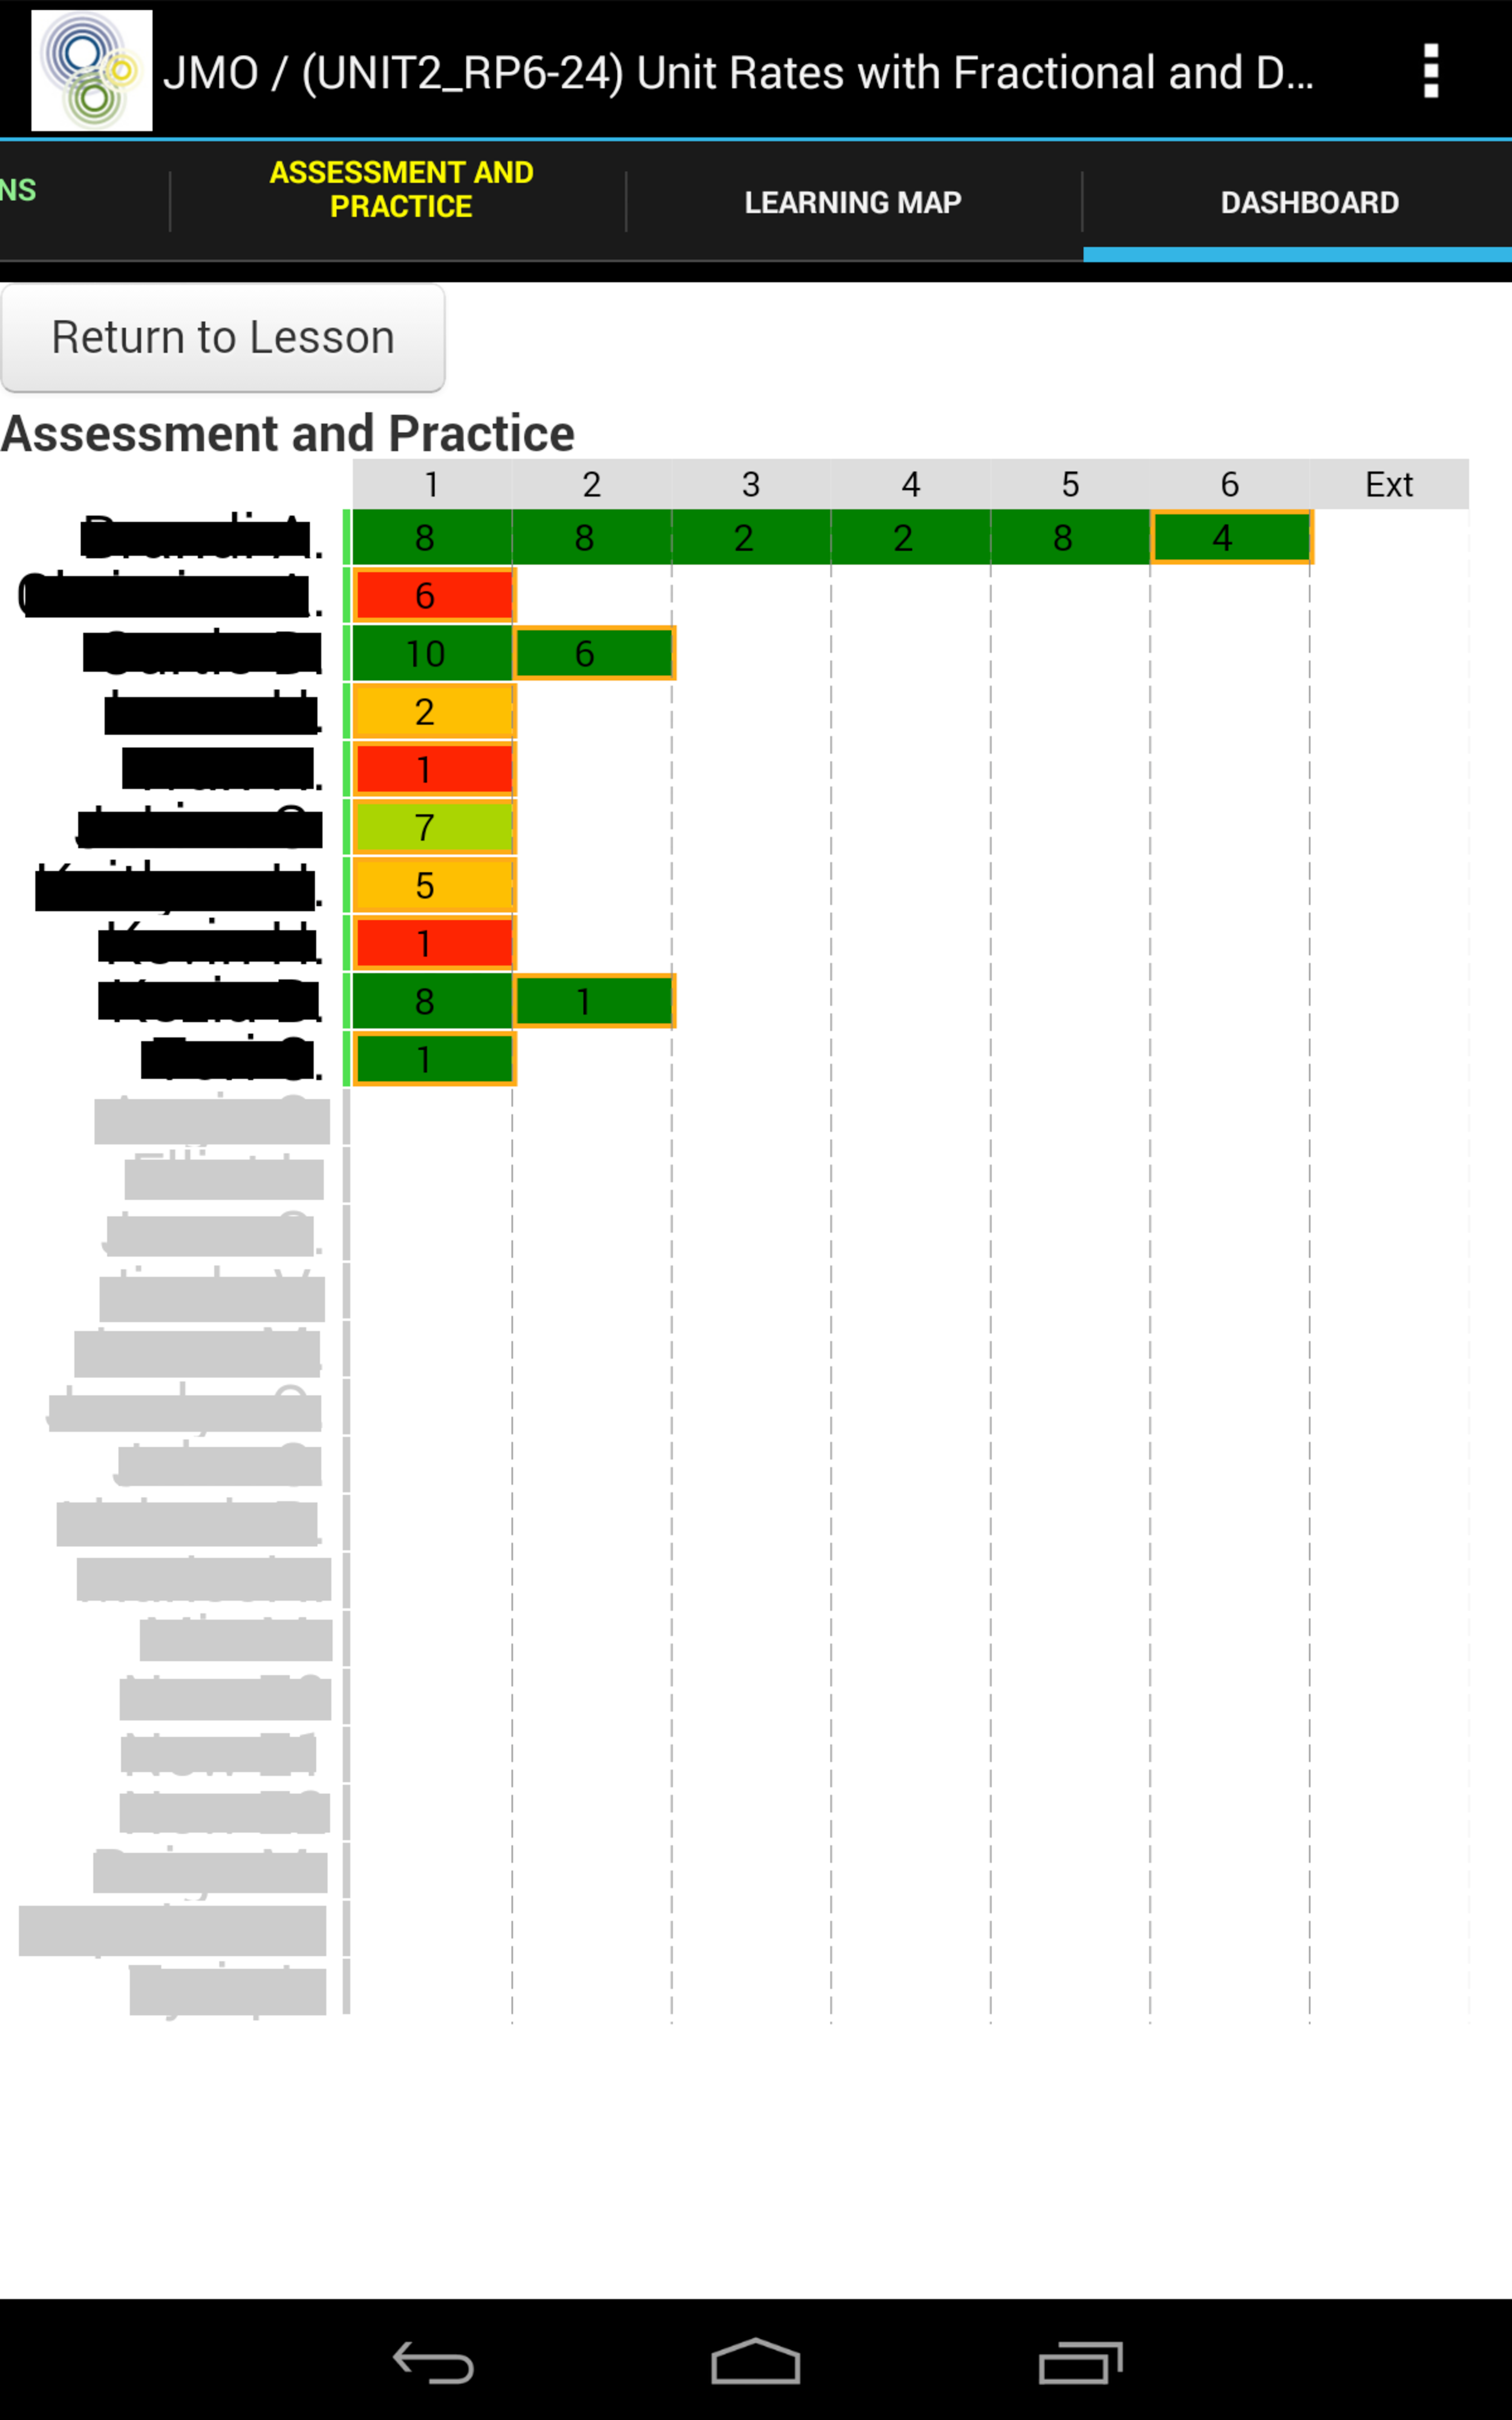
\includegraphics[width=40mm]{images/prior1.pdf}} \hspace{1em}%
\subfigure[]{\label{fig:Prior2}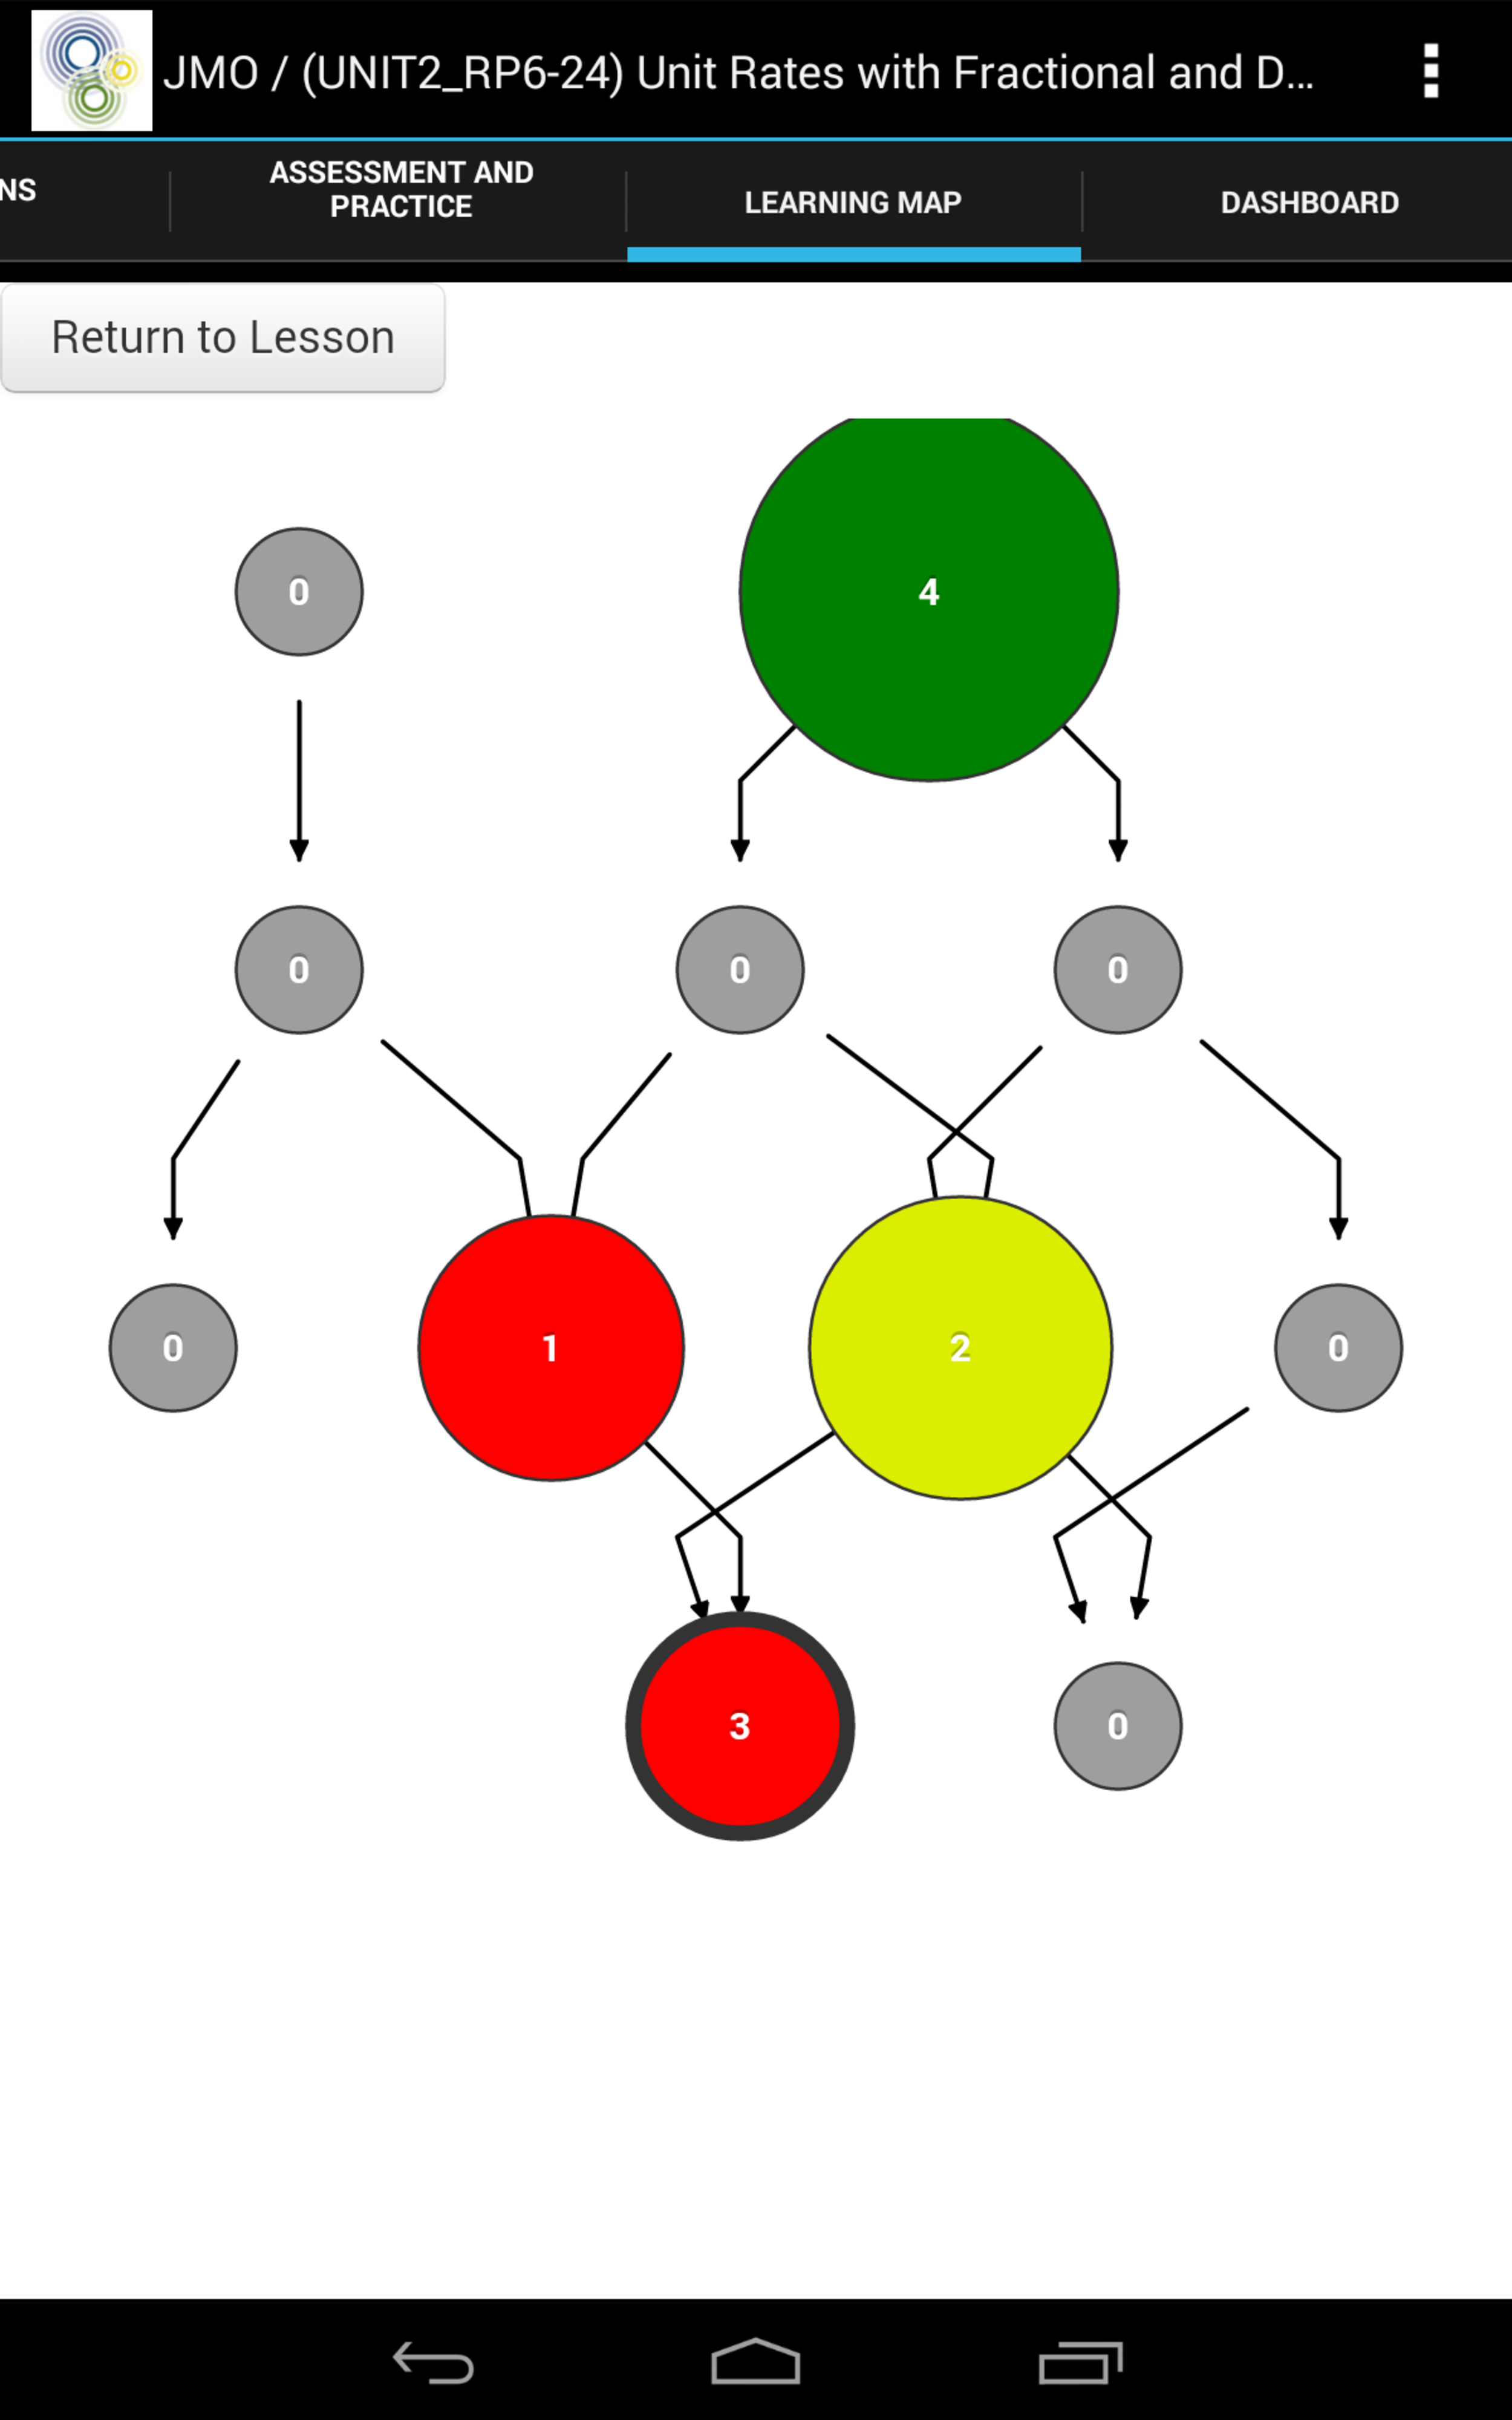
\includegraphics[width=40mm]{images/prior2.pdf}} \hspace{1em}%
\caption{Enlearn's initial attempts at visualizing student problem-solving data in real time. Figure (a) shows a table view of overall student performance over the course of the lesson. Figure (b) shows students organized by current concept. Both visualizations have design and usability flaws with regards to teacher needs, which motivates our work of creating create new, more appropriate visualizations.}
\label{fig:Prior}
\end{figure*}

\subsection{Enlearn's Existing Visualizations}

In the current teacher version of their software, Enlearn implemented two different methods of visualizing real-time student data. A week long trial conducted in classrooms this spring revealed that both designs have usability and readability problems. 

Enlearn's first design, shown in Figure \ref{fig:Prior1}, displays a table view of student problem-solving pace and correctness. While this visualization provides information about the progress of individual students, it communicates nothing about the specific concepts that students are struggling with. Enlearn's second design, shown in Figure \ref{fig:Prior2}, displays a graph view, organized by concept, of student problem solving. While this displays information about the concepts that students are generally struggling with, there is no way for teachers to view information on individual students nor to determine what they need assistance with. Most importantly, teachers are extremely busy during class time and need visualizations that are both easily glanceable and that provide actionable information - neither visualization provides good support in those areas.

Prior work shows the utility of communicating student data for instructors, and Enlearn's experiences with their current visualizations shows the challenge of designing effective means of communicating data in real-time for busy teachers. This motivates our desire to improve and build upon Enlearn's visualizations.

%While research shows that student data can help teachers understand misconceptions and how they spend class time, very little is known about how to visualize student data to most effectively communicate with teachers. We have not encountered any papers that study the design of visualizations of student data. Enlearn has implemented two different methods of visualizing student data in real-time for teachers, however, both of their designs have had usability and readability problems when tested in classrooms. This shows how challenging it is to create effective visualizations for communicating student data in real-time. Enlearn's first design, shown in Figure 1a, displays a table view of student problem solving pace and correctness. While this visualization provides information about the progress of individual students, it communicates nothing about the specific concepts that students are struggling with. Enlearn's second design, shown in Figure 1b, displays a graph view of student problem solving that is organized by concept. While this displays information about the concepts that students are struggling with, there is no way for teachers to see which individuals are struggling. Most importantly, neither visualization provides teachers with actionable suggestions about how to assist students who are struggling. Prior work shows the utility of communicating student data for instructors, and Enlearn?s experiences with their current visualizations shows the challenge of designing effective means of communicating data, especially in real time for busy teachers. This motivates our desire to improve and strengthen the data visualization for the Enlearn software.

%\section{Enlearn}
%For this project, we partnered with Enlearn, a non-profit company founded to develop tablet-based adaptive problem-solving software for K-12 classrooms. In our visualizations, we display real data from Enlearn students.

% Enlearn evaluated two visualizations with teachers this spring. One displays student data in a table view, but provides no concept-level information. The other displays a concept graph, but provides no data at the level of individual students.

% Enlearn found that neither visualization was effective in the classroom, in large part because the information provided did not match teacher needs. Another challenge is that teachers are extremely busy during class time and need visualizations that are both easily glanceable and that provide actionable information.

\section{Methods}
To address the challenge of designing effective techniques for visualizing student problem-solving data for teachers, we characterize the problem, discuss our data abstractions, present our visual encodings for conveying the data, and, lastly, describe our implementation.


\subsection{Problem Characterization}
The initial goal of this research was to understand the format of the problem-solving data collected by the Enlearn software and accurately characterize the tasks that teachers want to accomplish using this data. The challenges that Enlearn faced with their initial visualization designs shows the importance of understanding user needs; Enlearn's visualizations failed in large part because they did not effectively support teacher tasks. While we did not directly meet with teachers, we worked closely with Enlearn staff to understand the feedback they received in response to their initial visualizations. Here, we first describe the structure of the problem-solving data collected by Enlearn, and then describe teacher tasks. We provide a set of design guidelines for our visualizations based on this problem characterization.

\subsubsection{Enlearn Data Structure}
In Enlearn classrooms, each student solves problems on a personal tablet. Enlearn logs the following problem-solving information to a database: the id of the student, the id of the problem, the id of the associated problem set, the problem completion timestamp,  and whether or not the student answered the problem correctly. The Enlearn adaptive curriculum is designed as an extension of the JUMP Math curriculum \cite{JUMPMath}. In JUMP Math, students solve a linear progression of Exercise and Workbook problems. In Enlearn's adaptive version of the curriculum, students practice each type of Exercise or Workbook problem until they have mastered the concept covered by that problem. As a result, students may work on multiple practice problems of the type ``Exercise Problem 3'' before moving on to the next problem type. Enlearn refers to each problem type as a \emph{problem set}, but we use the term \emph{concept} in this paper since it better matches how teachers refer to the groups of problems.

\subsubsection{Teacher Tasks}
Through our discussions with Enlearn staff, we learned that there are two primary tasks that teachers want to accomplish using student problem-solving data during class. First, teachers want to determine which students need individual assistance and what specific concepts they are struggling with at any given moment. Ideally, teachers would also be able to see if multiple students are struggling with the same concept at the same time so that they can pull the students aside to work with as a group. Second, teachers want to determine how each student is performing overall during the current lesson. If many students are struggling with the content, the teacher may chose to re-teach parts of the lesson.

While Enlearn's initial visualizations tried to target these tasks, they did not provide adequate information for teachers to be able to quickly determine which students were struggling the most and what concepts they were currently working on. The overwhelming feedback that Enlearn was given by teachers after their trial was that the real-time visualizations need to provide information that is glanceable and immediately actionable. During class, teachers are busy adapting lessons, responding to students, and managing organizational challenges. They do not have time to explore a complex visualization of student data. Instead, they need a simple view that provides them with the exact information they need to accomplish in-class tasks such as assisting students and altering their teaching strategy.

\subsubsection{Design Guidelines}
From our characterization of the structure of Enlearn's problem-solving data and the tasks that teachers need to accomplish using that data, we developed the following design guidelines for our visualizations:

\begin{itemize} \itemsep5pt \parskip0pt \parsep0pt
  \item Visualizations must provide actionable information that clearly displays student performance on practice problems.
  \item Visualizations must show data for individual students so that teachers can easily intervene when needed.
  \item Visualizations must display concept-level data so that teachers can assess student understanding of each concept.
\end{itemize}

We use these guidelines throughout the remainder of our work to focus our data abstraction and visual encoding designs.

\subsection{Data Abstractions}
With our improved understanding of Enlearn's data structure and teachers' real-time visualization needs, we developed a set of data abstractions. First, we identify the set of low-level data \emph{operations} that need to be performed using the taxonomy developed by Amar, Eagan, and Stasko \cite{Amar05}. To assess student performance and determine which students are struggling, teachers must \emph{compute derived values} of student performance across multiple problems or concepts. To determine which concepts students are struggling with, teachers must also \emph{sort} students by concept. Finally, to quickly find individual students, teachers must \emph{sort} data alphabetically. Since teachers do not have time to perform these operations manually during class, our visualizations need to automatically compute averages and sort students.

The raw problem-solving data consists of the problem id, problem timestamp, problem correctness, student id, and concept id. We transformed this data into a nested JSON object that would make it possible to perform the necessary computations and sorting. First, we group problem data by student so that we can calculate how well each student is performing overall. With each student, we further group problem data by concept so that we can determine how well students perform on each concept. To capture information about how students spend their time, we calculate a start and end time for each concept. For each problem, we store problem correctness and the problem timestamp. This nested \emph{data type} allows us to compute the average performance of each student for both individual concepts and the entire lesson.

\begin{figure}[t]
\centering
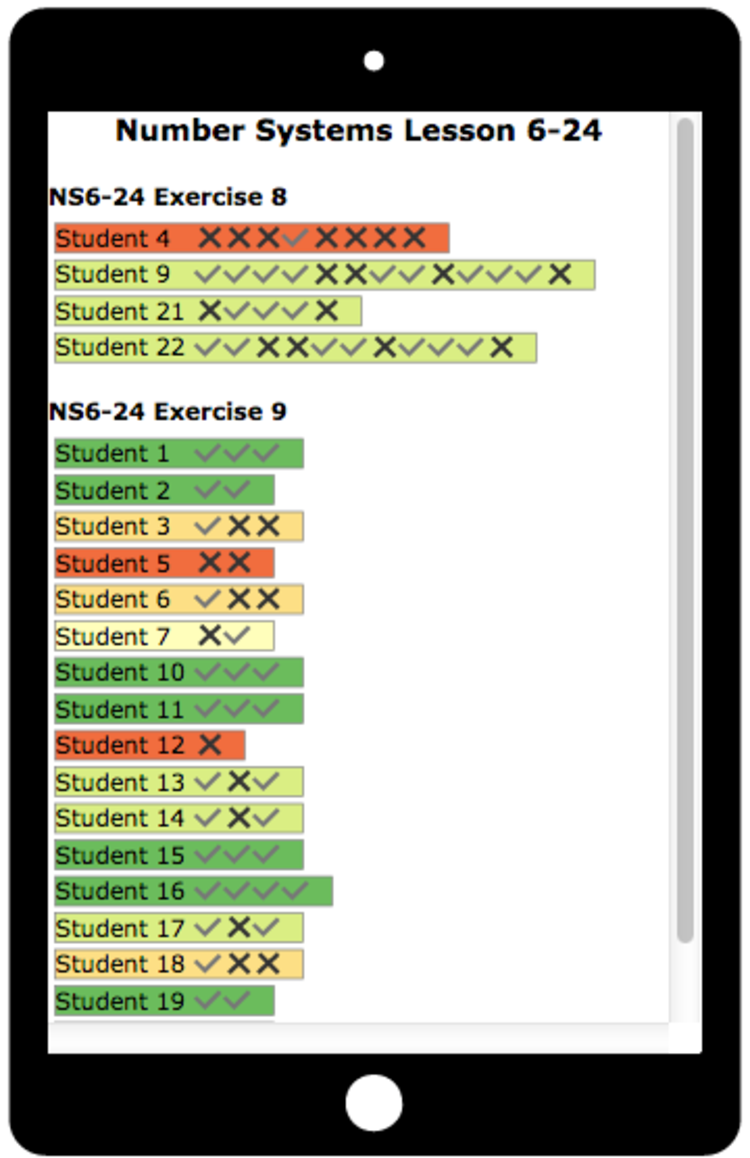
\includegraphics[width=55mm]{images/ConceptVisualization.pdf}
\caption{The concept visualization view. Students are grouped according to the current mathematical concept they are working on.}
\label{fig:ConceptVisualization}
\end{figure}

\begin{figure*}[t]
\centering
\subfigure[]{\label{fig:SummaryVisualization}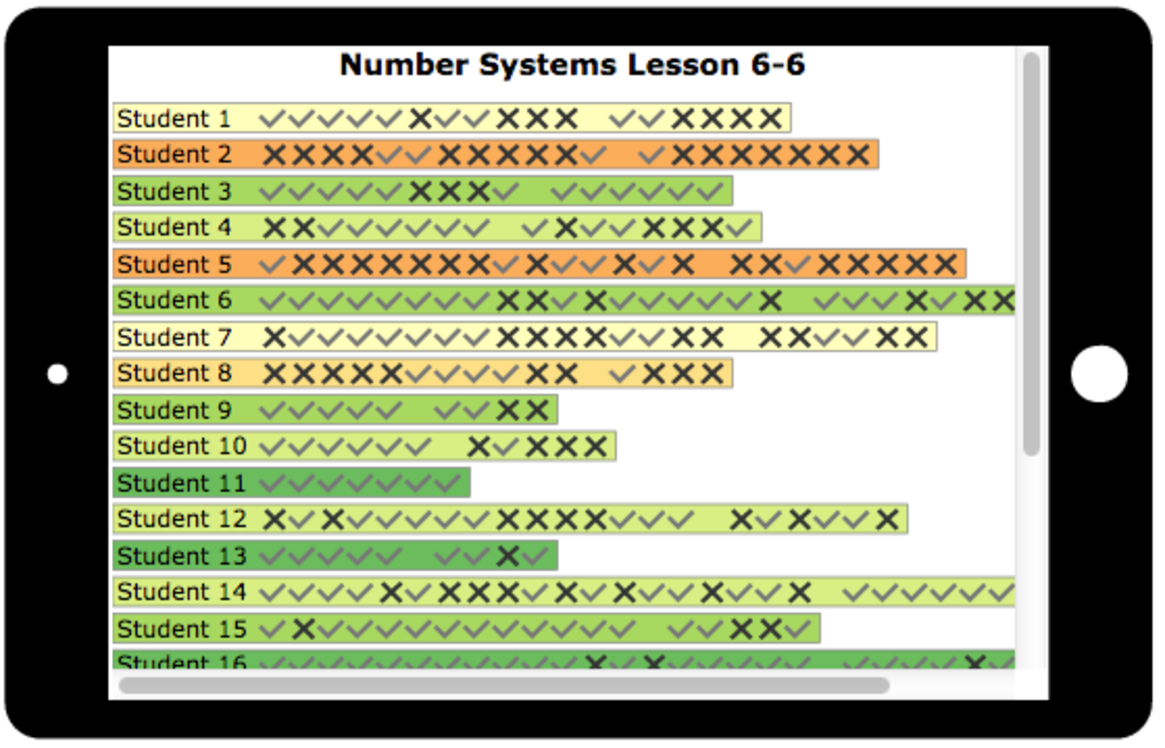
\includegraphics[width=80mm]{images/SummaryVisualization.pdf}} \hspace{1em}%
\subfigure[]{\label{fig:SummaryVisualizationClick}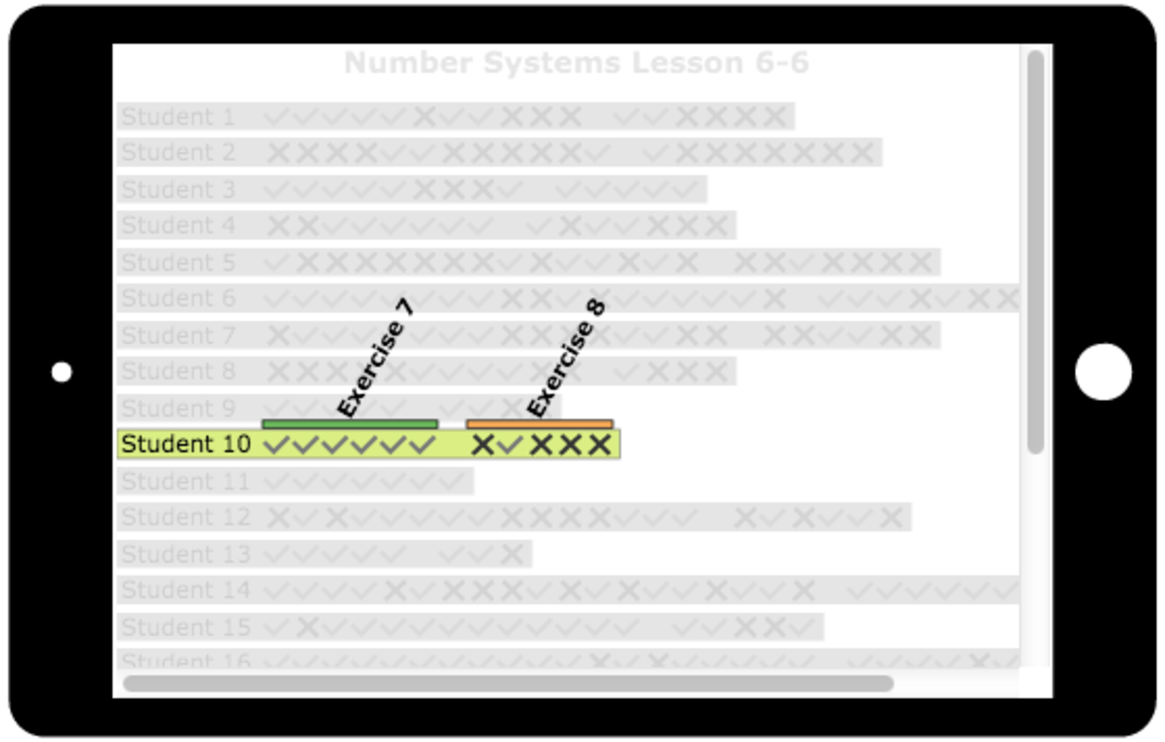
\includegraphics[width=80mm]{images/SummaryVisualizationClick.pdf}} \hspace{1em}%
\caption{Two views of the aggregate visualization. Figure (a) shows the overall aggregate view. Figure (b) shows the view after one of the student progress bars is tapped, bringing it into focus and displaying concept-level information on problem correctness. }
\label{fig:Spreadsheet}
\end{figure*}



\subsection{Visual Encodings}
To support the tasks that teachers want to accomplish using student problem-solving data during class time, we developed two separate visual encodings. We describe the goals and structure of each visual encoding below, and then discuss our visual design choices in detail.

\subsubsection{Concept Visualization}
We designed the concept visualization to help teachers determine which students need individual assistance in the present moment. In this visualization, students are sorted first by concept and then alphabetically. For each student, we display a bar showing problem-solving information for the concept that the student is currently working on. The bar shows check marks for correct problems and cross marks for incorrect problems, indicating both the number of problems a student has completed for this concept and problem correctness. The bar is colored according to the student's average performance on the concept. A screenshot of the concept visualization can be seen in Figure \ref{fig:ConceptVisualization}.

The goal of this visual encoding is to allow teachers to rapidly identify students who are struggling. One issue with the visualizations that Enlearn tested was that it was difficult for teachers to determine which specific concepts were currently struggling with. By grouping students by concept, we expose this concept-level information and make it possible for teachers to provide targeted assistance. Furthermore, this encoding makes it straightforward for teachers to determine if multiple students are struggling with the same concept. Teachers may choose to work with these students in small groups or re-teach the concept to the entire class based on this concept-level performance information.

\subsubsection{Aggregate Visualization}
We designed the aggregate visualization to give teachers a high-level overview of how students are performing during the current lesson. In this visualization, students are sorted alphabetically. For each student, we display a bar showing all of the student's problem-solving information for the current class period. Again, the bar shows check and cross marks to indicate problem correctness. We leave a blank space between the marks for separate concepts to visually separate them. The bar is colored according to the student's average performance during this class period. A screenshot of the aggregate visualization can be seen in Figure \ref{fig:SummaryVisualization}.

The goal of this visual encoding is to allow teachers to assess student's overall performance during the current lesson. In Enlearn's initial studies, teachers found the table summary visualization most useful, so we wanted to create something similar. With this encoding, we make it possible for teachers to identify students who are performing poorly or who have completed fewer problems. If students are performing poorly across the board, teachers may decide to stop problem solving and re-teach lesson content. 

While the aggregate performance information provides a high-level summary for teachers, we also wanted to make concept-level information accessible through the aggregate visualization. We added an interactive feature to this visualization, allowing the teacher to access concept-level information for a given student by clicking on the student's bar, as shown in Figure \ref{fig:SummaryVisualizationClick}.

\begin{figure}[t]
\centering
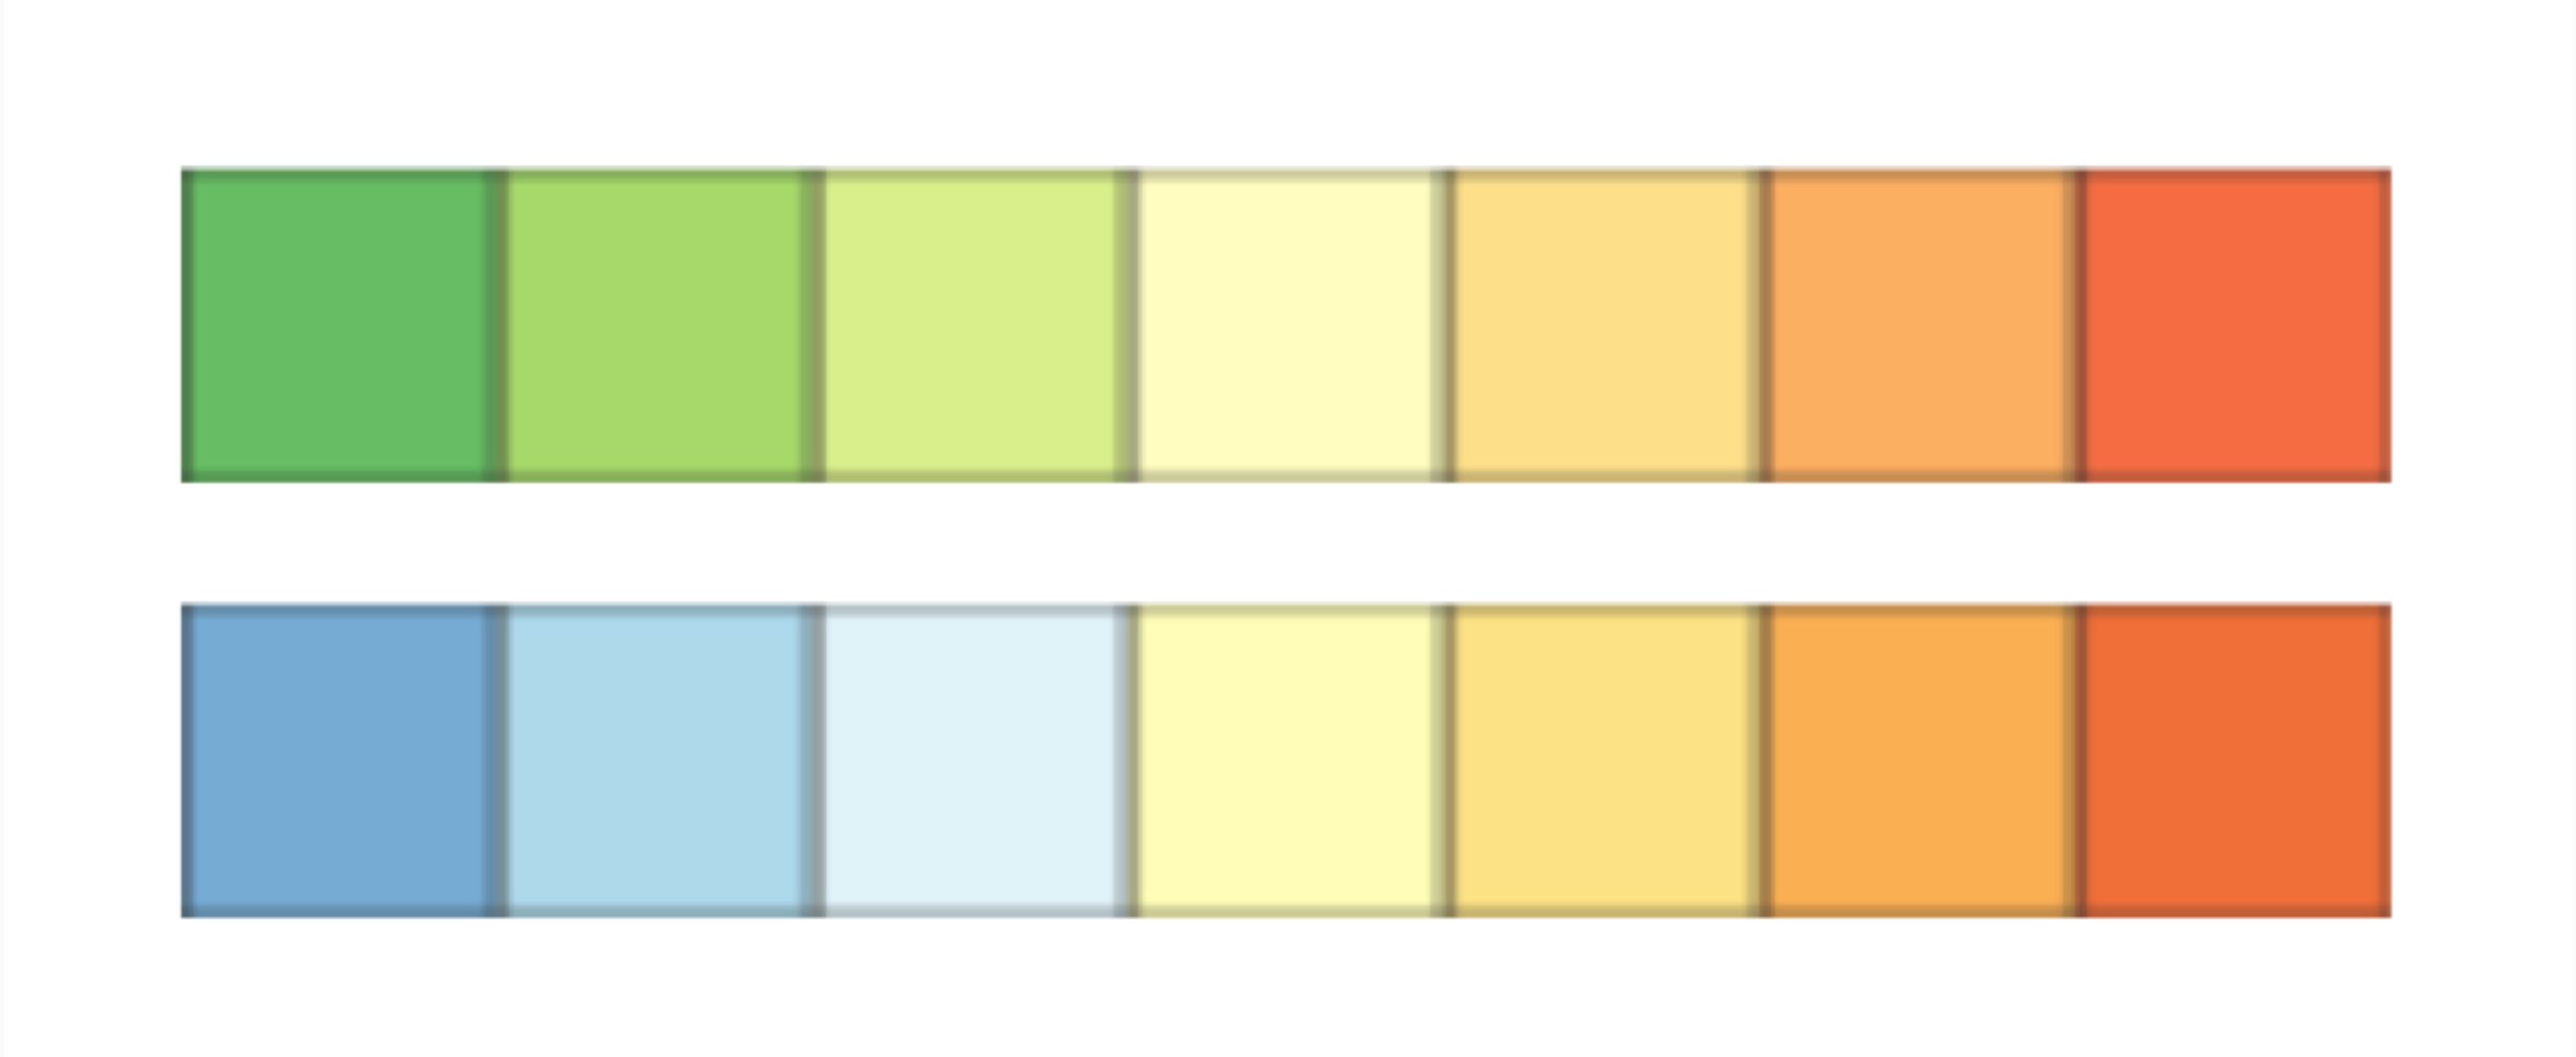
\includegraphics[width=65mm]{images/ColorGradients.pdf}
\caption{The color gradients used to denote the percentage of problems a student has answered correctly. We include both a red-green scale to match common encodings of correctness, and a red-blue scale for color-blind viewers.}
\label{fig:ColorGradients}
\end{figure}

\subsubsection{Visual Design}
In both visualizations, we display one horizontal bar per student that shows problem-solving information. We chose to use the common encoding of check marks and cross marks to denote problem correctness, and display marks in a neutral gray color that stands out against the bar background. Identifying incorrect responses is most important for teachers for the purpose of real-time intervention, so we color crosses in a darker gray than checks to increase their visual significance.

We color the background of each student bar based on average problem correctness. By default, we use a seven-step gradient of colors that ranges from a red to a  green with yellow as the midpoint. We chose this encoding because red and green are commonly used to denote correctness in educational settings. While this encoding is the most natural for most teachers, it is not an appropriate gradient for color blind users. To provide support for color blind teachers, we include an option for switching to an orange-blue color gradient if desired. Our color gradients are shown in Figure \ref{fig:ColorGradients}. We selected our these colors using ColorBrewer \cite{ColorBrewer}, an application designed to provide a range of easily differentiable color schemes.

Our visualizations are designed to be used in real-time with streaming data. This means that the displayed data is constantly changing. We use animation in both visualizations to smooth transitions and signify changes. This is particularly important in the concept visualization, since students move dynamically between concepts. We gradually fade student bars in and out when students move between concepts to make these transitions more gradual and visible. %We chose to not use transitions to add new check and cross marks.

\subsection{Implementation}
In this work, we focused on characterizing the data visualization needs of classroom teachers, developing appropriate data abstractions, and designing visualizations to target teacher needs. Our end goal was not to produce fully functional visualizations that integrate with real-time data streams and run on tablet devices; instead, we wanted to create an environment that Enlearn staff could use to explore and evaluate our designs. We therefore decided to simulate how our visualizations would look on tablet computers with streaming data. This approach will allow us to rapidly iterate on our designs with Enlearn staff before implementing a final production-level product.

We used the D3 visualization library to create our visualizations. Enlearn's current data visualizations are also implemented with D3, so this approach is compatible with their current workflow. In the following sections, we describe how we simulate the tablet interface and streaming data, and discuss the design of our final system.

%Image dump can go here
\begin{figure*}[t]
\centering
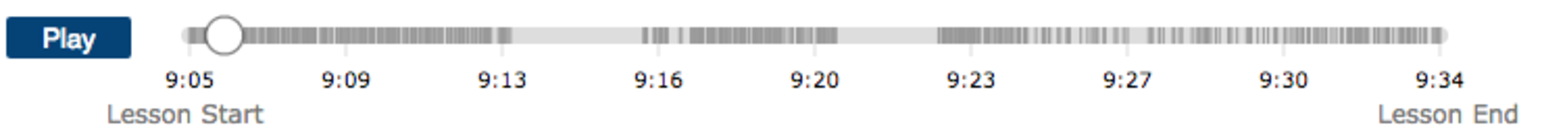
\includegraphics[width=180mm]{images/Timeline.pdf}
\caption{Since we do not have access to real-time student problem-solving data, we simulate data streaming using this timeline slider. Users can play back and brush through data to reenact the progression of a single lesson.}
\label{fig:Timeline}
\end{figure*}

\subsubsection{Tablet Graphic}
To simulate how our visualizations would appear on a teacher tablet, we display the visualizations within a tablet graphic on our website. The tablet's display area is restricted to the dimensions of the graphic, and users can scroll as they would on an actual device. We display the concept visualization in a vertically positioned tablet and the aggregate view in a horizontally positioned tablet. The concept view is typically longer than it is wide, while the aggregate view is wider than it is tall. We chose these orientations to maximize the amount of visual information. When the user switches between the two visualizations, we rotate the orientation of the tablet graphic. We use animated transitions to reduce any jarring effect of switching between orientations.

\subsubsection{Simulating Streaming Data}
To simulate how our visualizations would appear with real-time streaming data, we use a timeline interface to allow users to play and scrub through previously collected data. This approach allows users to both experience the visualizations as they would appear with real-time streaming data and advance to interesting events to quickly assess the visual design. We display lines on the timeline bar to indicate where problem-solving actions occur. These visual information scent cues \cite{Willett07} are designed to help users become familiar with the data set. This is particularly important for our data because there are often long gaps in problem-solving when teachers pause students to clarify a concept or walk through an example. A screenshot of the timeline is shown in Figure \ref{fig:Timeline}. While we designed the timeline for our benefit as designers, initial feedback suggests that this type of interaction could be valuable for teachers as well. We discuss this further in Future Work.

\subsubsection{Website Design}
We designed our final website to display all information in a single screen, and sized content for optimal viewing on a screen with resolution least 1280px by 800px. We display the timeline at the top of the page, and auto-play the simulated data stream on load. Beneath the timeline we display the tablet graphic and the current visualization. To the right-hand side of the screen, we display textual information about the visualization to provide some context for new users. We provide buttons for changing visualization options inline with descriptions about the features of each button. When a user clicks the ``Switch View'' button, the tablet graphic switches between the concept and aggregate visualizations. The textual information associated with the visualization changes as well. We also provide an option for the user to switch between five different data sets of real class sessions. Finally, we provide an option for switch between our two color schemes.  A screenshot of our final website is shown in Figure \ref{fig:Website}. 

\section{Results \& Discussion}
%The visualizations your system produces and data to help evaluate your approach. For example you may include running times, or the time users typically spend generating a visualization using your system.
%What has the audience learned from your work? What new insights or practices has your system enabled? A full blown user study is not expected, but informal observations of use that help evaluate your system are encouraged.

In this work, we have made contributions at multiple levels of Munzner's nested model of visualization design \cite{Munzner09}. We contribute a characterization of the real-time data visualization needs of classroom teachers, describe an appropriate data abstraction designed, and present two new visual encodings of student problem-solving data designed to target teacher needs. Screenshots of our final visualization designs are shown in Figure \ref{fig:Website}.

The primary goal of this work was to present our final visualization designs in an environment that would allow Enlearn staff and teachers to explore and evaluate the designs before implementing production-level versions of the visualizations for use in the classroom. While we have not formally evaluated our visualization designs yet, we collected informal feedback both from Enlearn staff and from attendees of the CSE 512 poster sessions. Overall feedback has been positive; Enlearn staff expressed excitement about the potential of these new visual encodings, and poster session attendees liked the visual designs and expressed an interest in the problem space.

While feedback was generally positive, we received a number of suggestions for improvements and revisions to our designs. Both Enlearn staff and poster session attendees questioned the utility of the aggregate visualization. At the poster session, a number of people suggested that we remove the problem-level checks and crosses, and instead display a grid of colors showing how each student performed on each concept. This would allow teachers to view overall student understanding at the concept level. Interestingly, Enlearn staff gave opposing feedback. The suggested that we color student bars based on recent progress rather than progress across multiple concepts. They reiterated the fact that the primary goal of teachers during class is to rapidly determine which student needs help \emph{right now}, and that they are not interested in viewing summary information during class time. This tension highlights the need for separate visualization designs to target in-class and after-class tasks.

Another suggestion that we heard from both Enlearn staff and poster session attendees is that the concept visualization may not adequately highlight struggling students. One suggested that we add a toggle to hide student who are performing well, so that teachers can focus on the students who need assistance. Another suggested that we sort bars by color to visually group struggling students. An Enlearn staff member also recommended that we wait to color student bars until at least three problems have been completed. In our current design, a single incorrect problem results in a striking red bar even though the student should try a few more times before receiving help. All of these options could improve the ease with which struggling students can be identified.

Finally, a number of people mentioned that the movement of students between concepts in the concept visualization could be jarring. If a teacher is watching the progress of a single student and that student suddenly disappears to another part of the visualization, it could be confusing. At the same time, students only move on to a new concept once they have mastered the previous one, so it is unlikely that struggling students will disappear. However, it is possible that a visualization that provides a persistent view of students but that provides filtering options to help teachers identify struggling students could be most effective.

One surprising result was that Enlearn staff were very excited about the possibility of providing teachers with the timeline interface so that they could review lessons after-the-fact. Staff members are also interested in using this interface to explore data from their studies; they have a mountain of log data from their 10-week trial this fall, but it is difficult to get a sense for how class time was spent and how students performed by looking at problem-solving data in aggregate. While we originally designed this interface to simulate a real-time data stream, it provides an interesting contribution in its own right.

Many of these design questions must be further explored by evaluating the visual designs with teachers, which we aim to address in future work. Despite these suggestions for improvements and extensions to our designs, overall feedback was very positive. At the poster session there was a lot of interest in the problem of visualizing student data; one attendee said that his mom is a middle-school teacher, and that he thinks she would love to have access to this type of real-time student data. Many others were interested in ways that our approaches could be extended to support large lecture classes or MOOCs. This seems like a ripe area for future research.

%Our final product is a visualization that integrates our concept view and aggregate views, playing back student progress over a math lesson via a timeline slider that supports brushing. Prior work displays student data at an assignment level, which does not afford immediate intervention in the classroom (may be a wild claim, must confirm). Our system simulates real-time, problem level visualizations that teachers can use to track student problem-solving progress. Through the concept view, teachers can immediately see which students need assistance and what to assist them with, and through the aggregate view, teachers can monitor longer term student progress over the course of a lesson. 

%On a more general level, our work is not limited to playing back data gathered from Enlearn math tablets. Any data set with information about problem time completion, problem correctness and problem concept grouping could be visualized using our tool.

%Overall, attendees of the CSE 512 project poster session reacted positively, commenting that our system was visually clean and easy to understand. One viewer mentioned that he taught middle school students and would find our visualization useful for tracking their progress. %Nell, can confirm? I think it was Kevin who said it

%Image dump can go here
\begin{figure}[t]
\centering
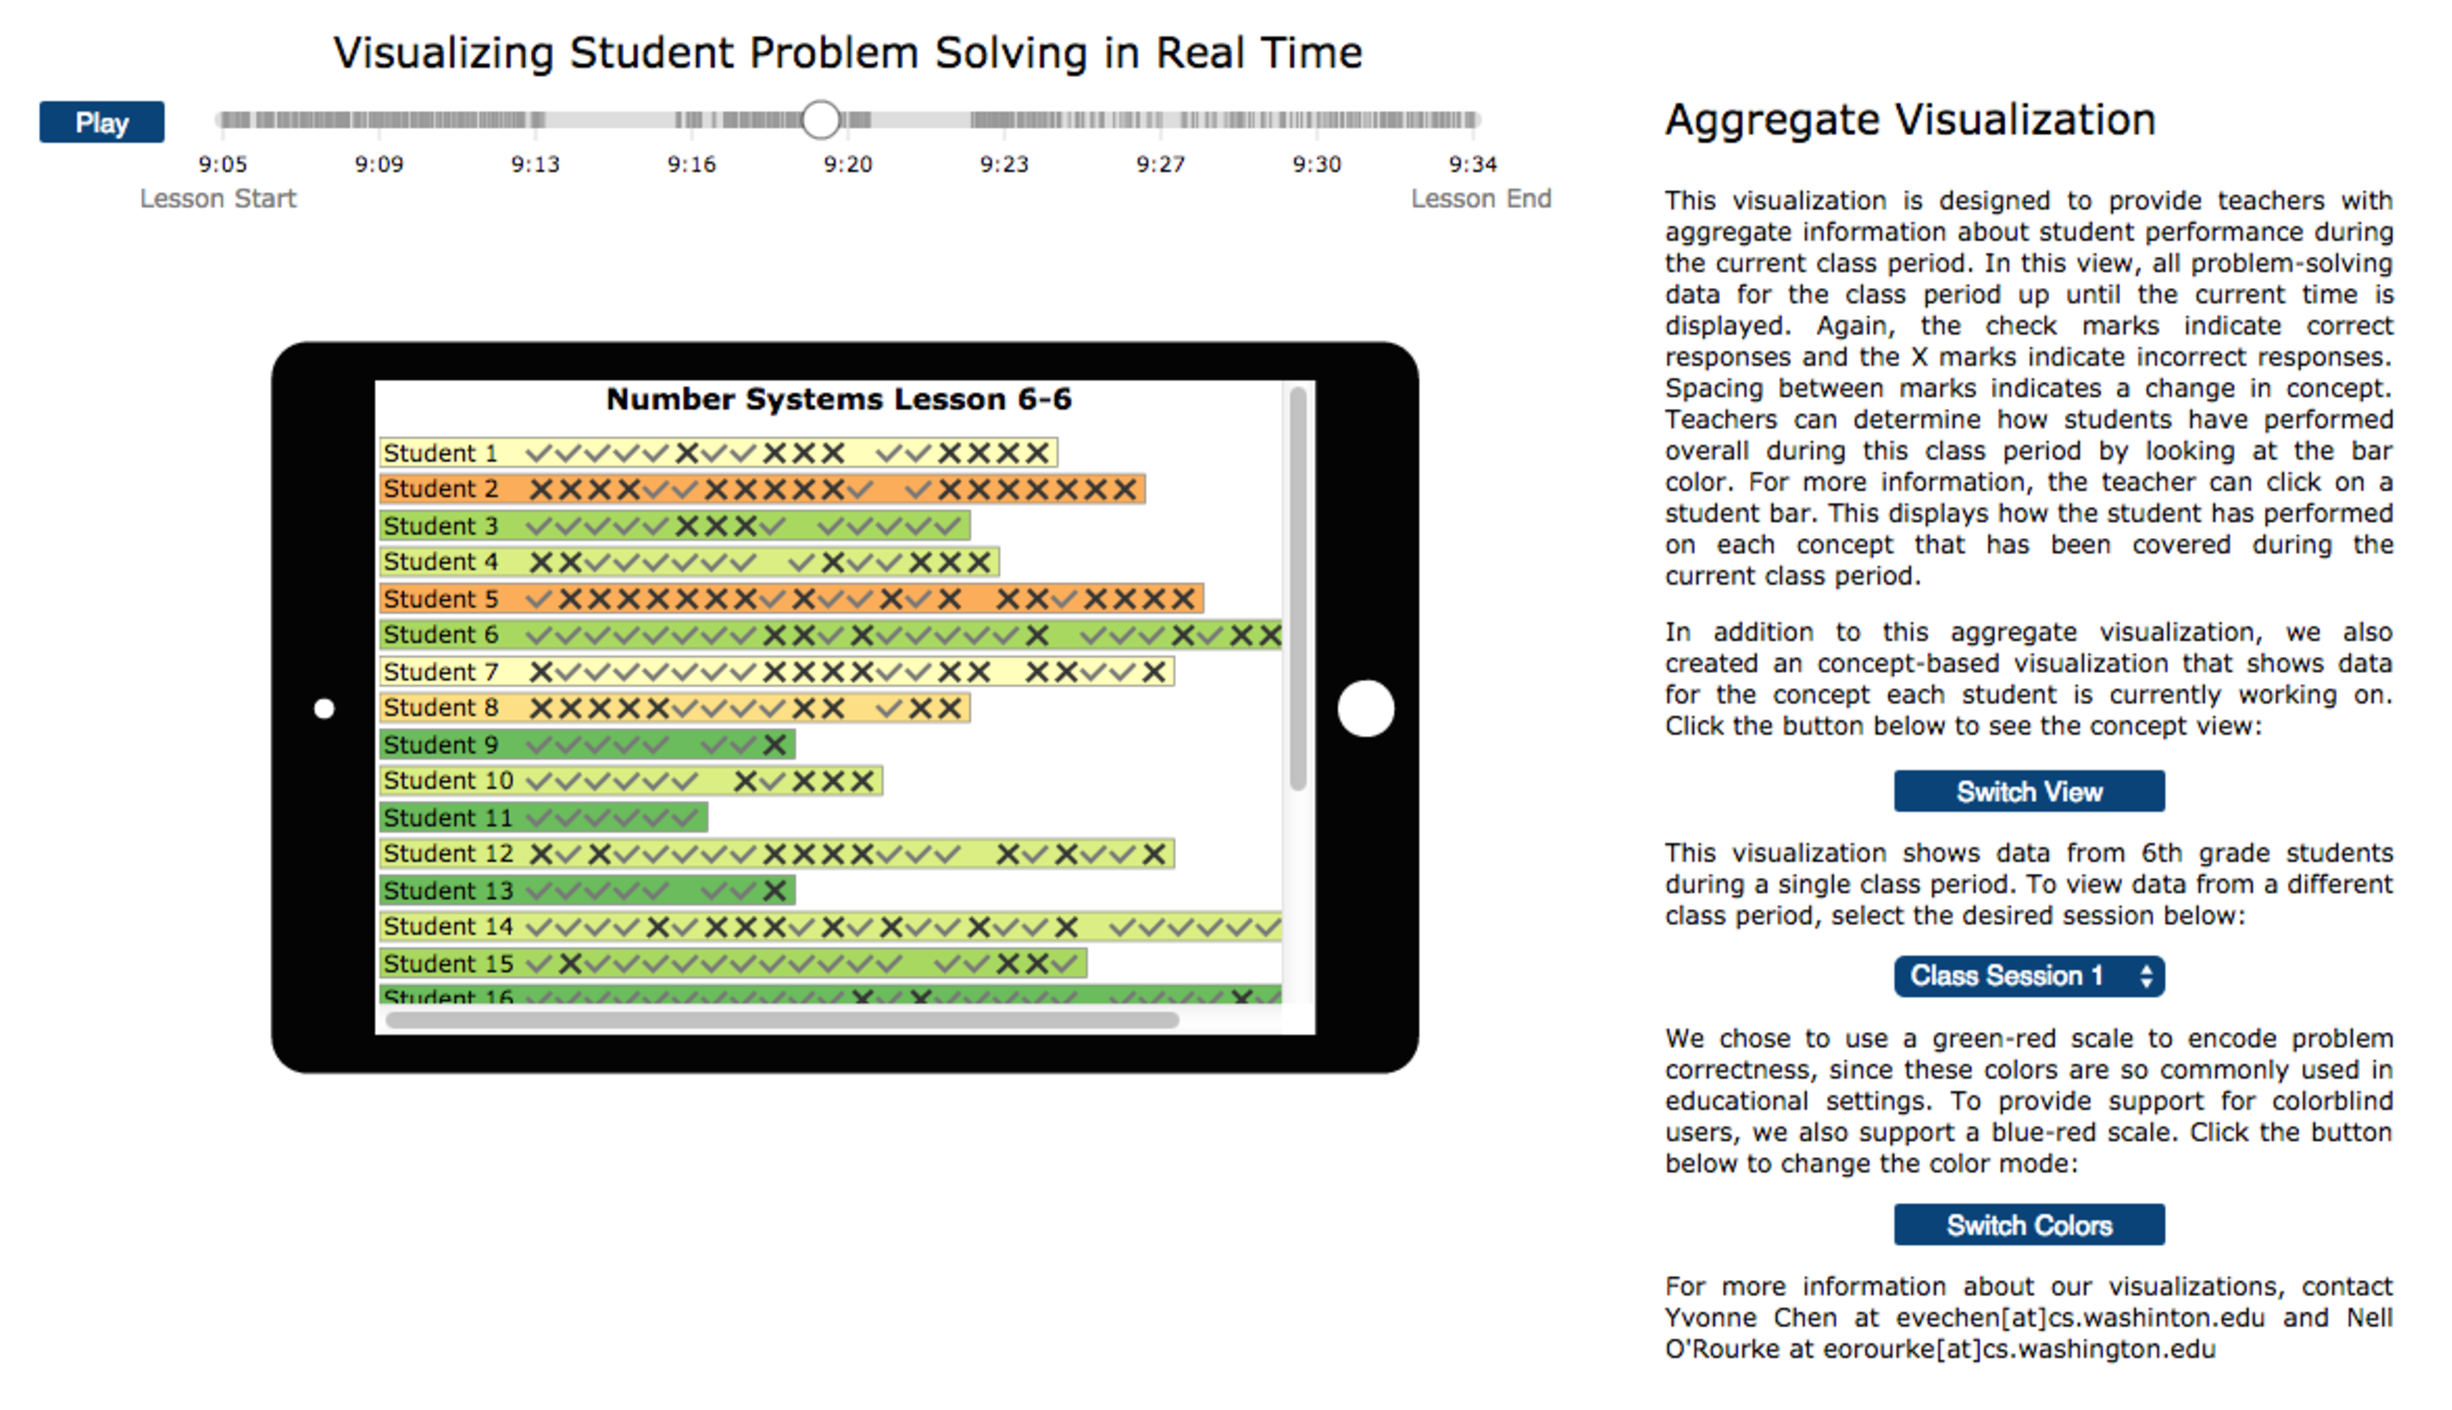
\includegraphics[width=65mm]{images/results1.pdf}
\caption{Our final visualization, shown displaying the summary view.}
\label{fig:Website}
\end{figure}

\section{Future Work}
%A description of how your system could be extended or refined.

There are a number of areas for future work. First, we need to evaluate our visualization designs with teachers and iterate on our designs. The informal feedback that we received from Enlearn staff highlights a number of open design questions that are difficult to answer without getting feedback from our target users. We would like to first iterate on our designs with the feedback we have received thus far, and then perform an informal evaluation of our simulated designs with teachers to help us further improve the designs. After these initial iteration cycles, we plan to work with Enlearn to port our D3 visualizations onto their platform so that we can formally evaluate our visualization designs in real classroom settings.

In addition to formally evaluating our real-time designs, we are also interested in exploring some of the alternative visualization designs suggested in the feedback we received. We are excited about the prospect of using the timeline interface to help visualize how class time is spent. In Enlearn classrooms, teachers use a tablet-based version of the curriculum teacher's guide to walk through lessons, example problems, and activities. All of this information is logged to Enlearn's databases. This type of data could be overlaid with the timeline slider to provide a complete picture of how class time is spent and how students perform. This could provide valuable insight for both teachers and researchers.


%As described above, the visual information scent cues overlaid on our timeline slider help inform viewers of gaps where students were not completing tablet problems. The teacher version of Enlearn's software collects data on teacher actions, such as sending a pause signal to freeze all student tablets to get their attention, or switching between lessons. Such information could be overlaid with the timeline slider as insight to teachers. For example, this feature could show that during a time when the teacher is talking, some problem solving activity is still present. This means some students  are off task and using their tablets instead of paying attention to their teacher. However, there is currently no feature to tell which student is associated with which tick marks. Calling out a student's associated tick marks when their name is clicked in the aggregate view would help teachers to monitor an individual student's activity patterns.
%
%Multiple visitors to the poster session that our aggregate view was not as easily glanceable as the concept view. They all independently suggested that information about each student's progress over a single concept could be collapsed into a single representative glyph, such as a shape colored to represent correctness. This way, all students' data could be displayed in a matrix, with pertinent information readily visible at a glance and detailed information accessible by tapping on the student's name. 
%
%Another comment received during the poster session was that our animation transitions could be clearer to help teachers track the movement of students between concepts.
%
%Although the above suggestions have potential to improve our work, an important next step is to evaluate our system with actual teachers. Enlearn has a preexisting relationship with Seattle school teachers, with whom they have collected tablet data over multiple trials. Since Enlearn's current visualizations are also created in D3.js, we can port our system into their software, to be evaluated in future classroom trials. Suggestions from the target audience are invaluable to substantial improvements to our work.

\section{Conclusion}
Our work makes multiple contributions to the field of student data visualization. We have identified a set of design guidelines for real-time data visualizations for teachers based on our characterization of the problem space. These guidelines focus on the importance of providing actionable information for teachers and presenting data at both the student and concept level. We characterize the operations that need to be performed on problem-solving data to address teacher needs, specifically \emph{sorting} and \emph{computing} average performance. Finally, we present two new visual encodings for student data, one that displays information for the concepts students are working on in the present moment, and another that displays aggregate performance across multiple concepts.



%\begin{figure*}[t]
%\centering
%\subfigure[]{\label{fig:TeacherLesson}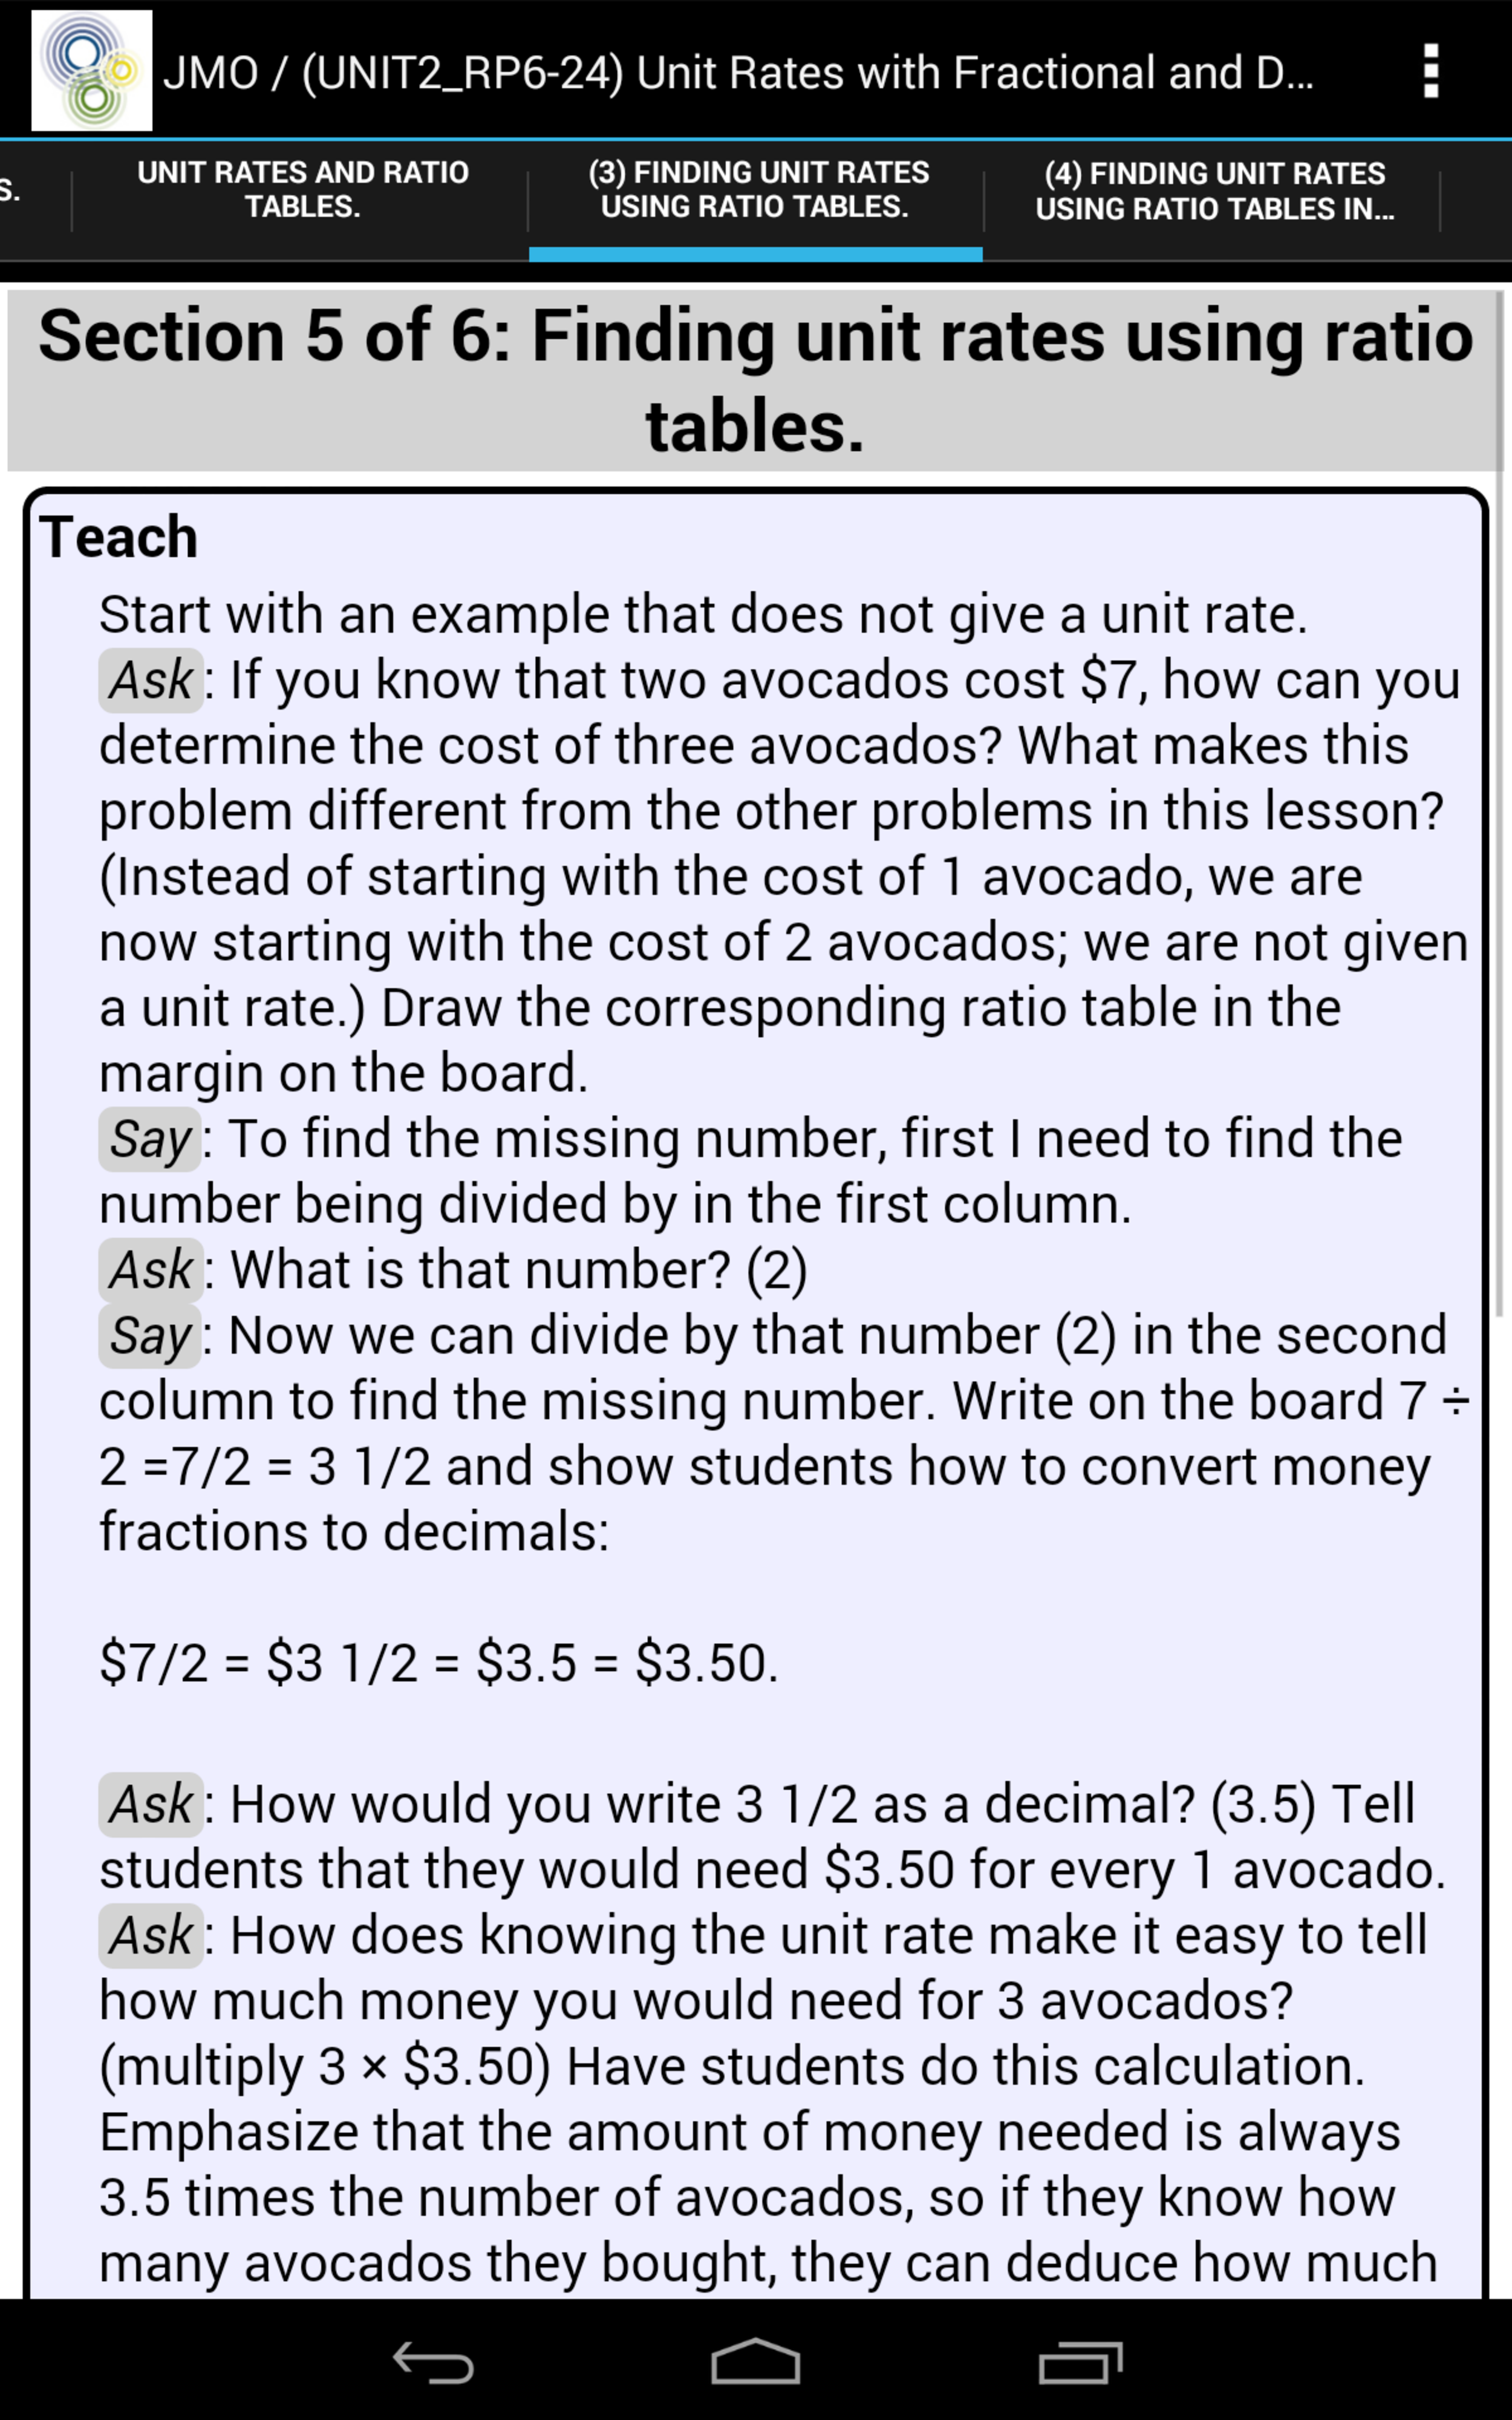
\includegraphics[width=40mm]{images/TeacherLesson.pdf}} \hspace{1em}%
%\subfigure[]{\label{fig:TeacherStartProbems}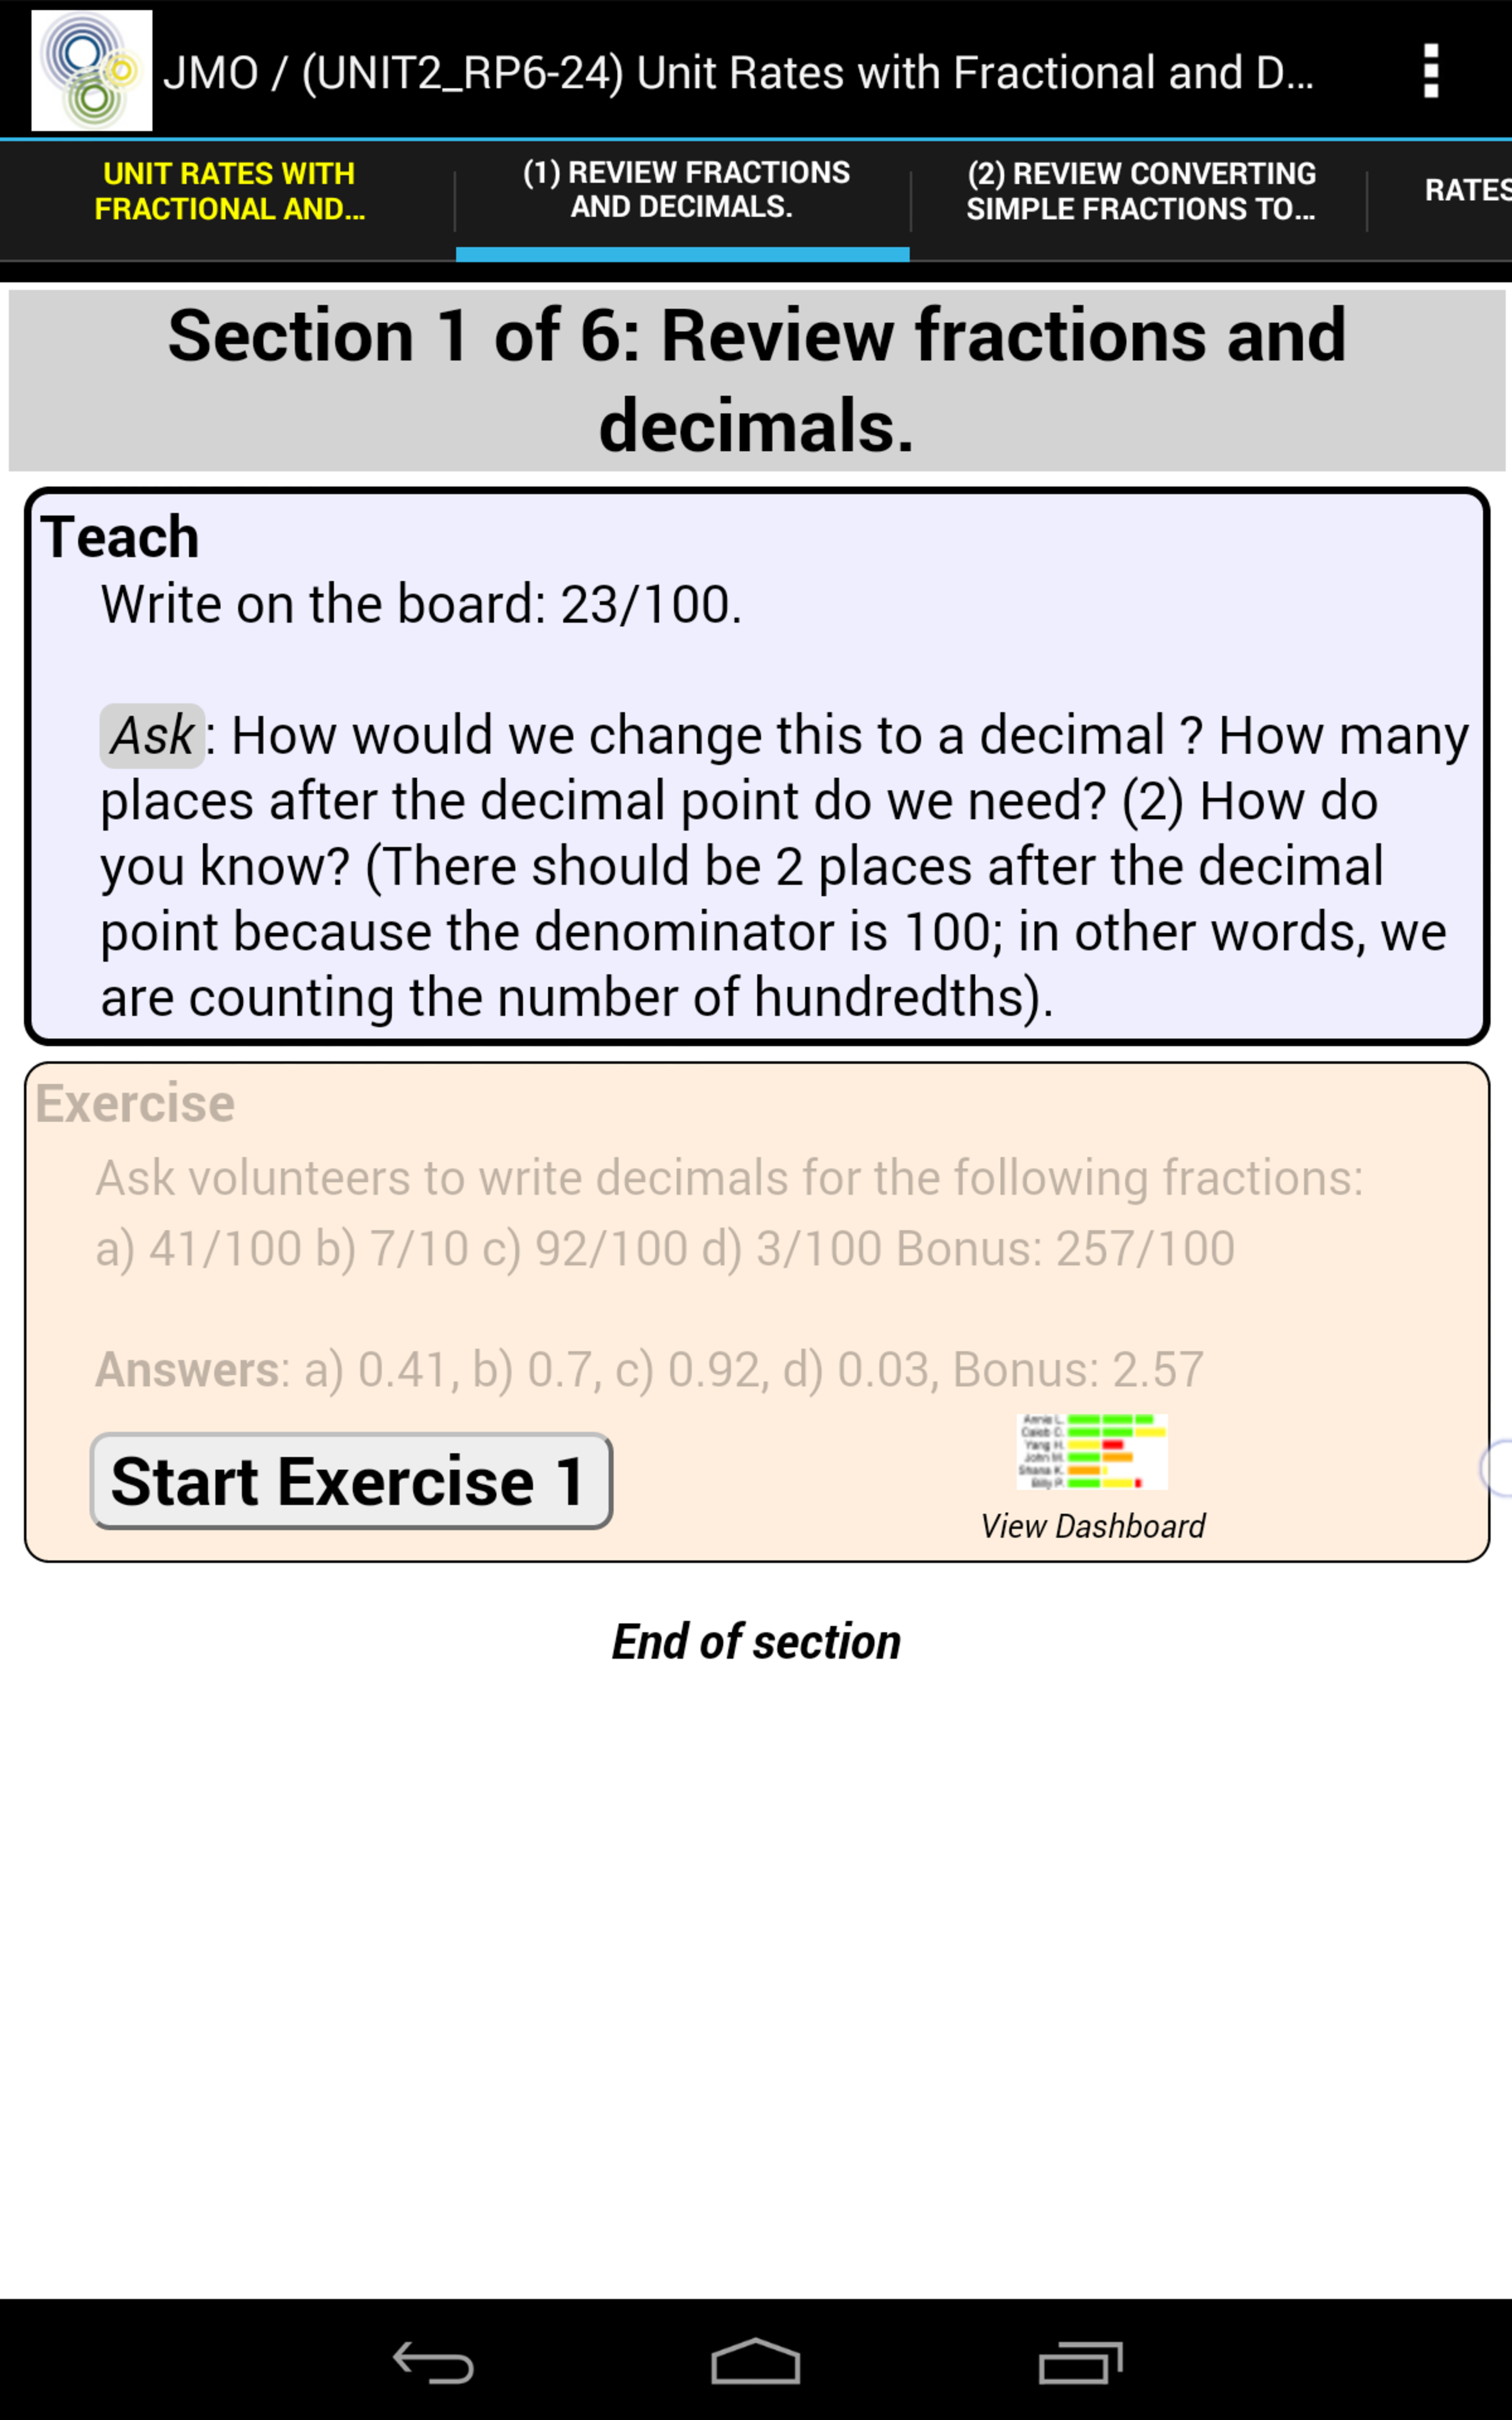
\includegraphics[width=40mm]{images/TeacherEX.pdf}} \hspace{1em}%
%\subfigure[]{\label{fig:TeacherDashboard}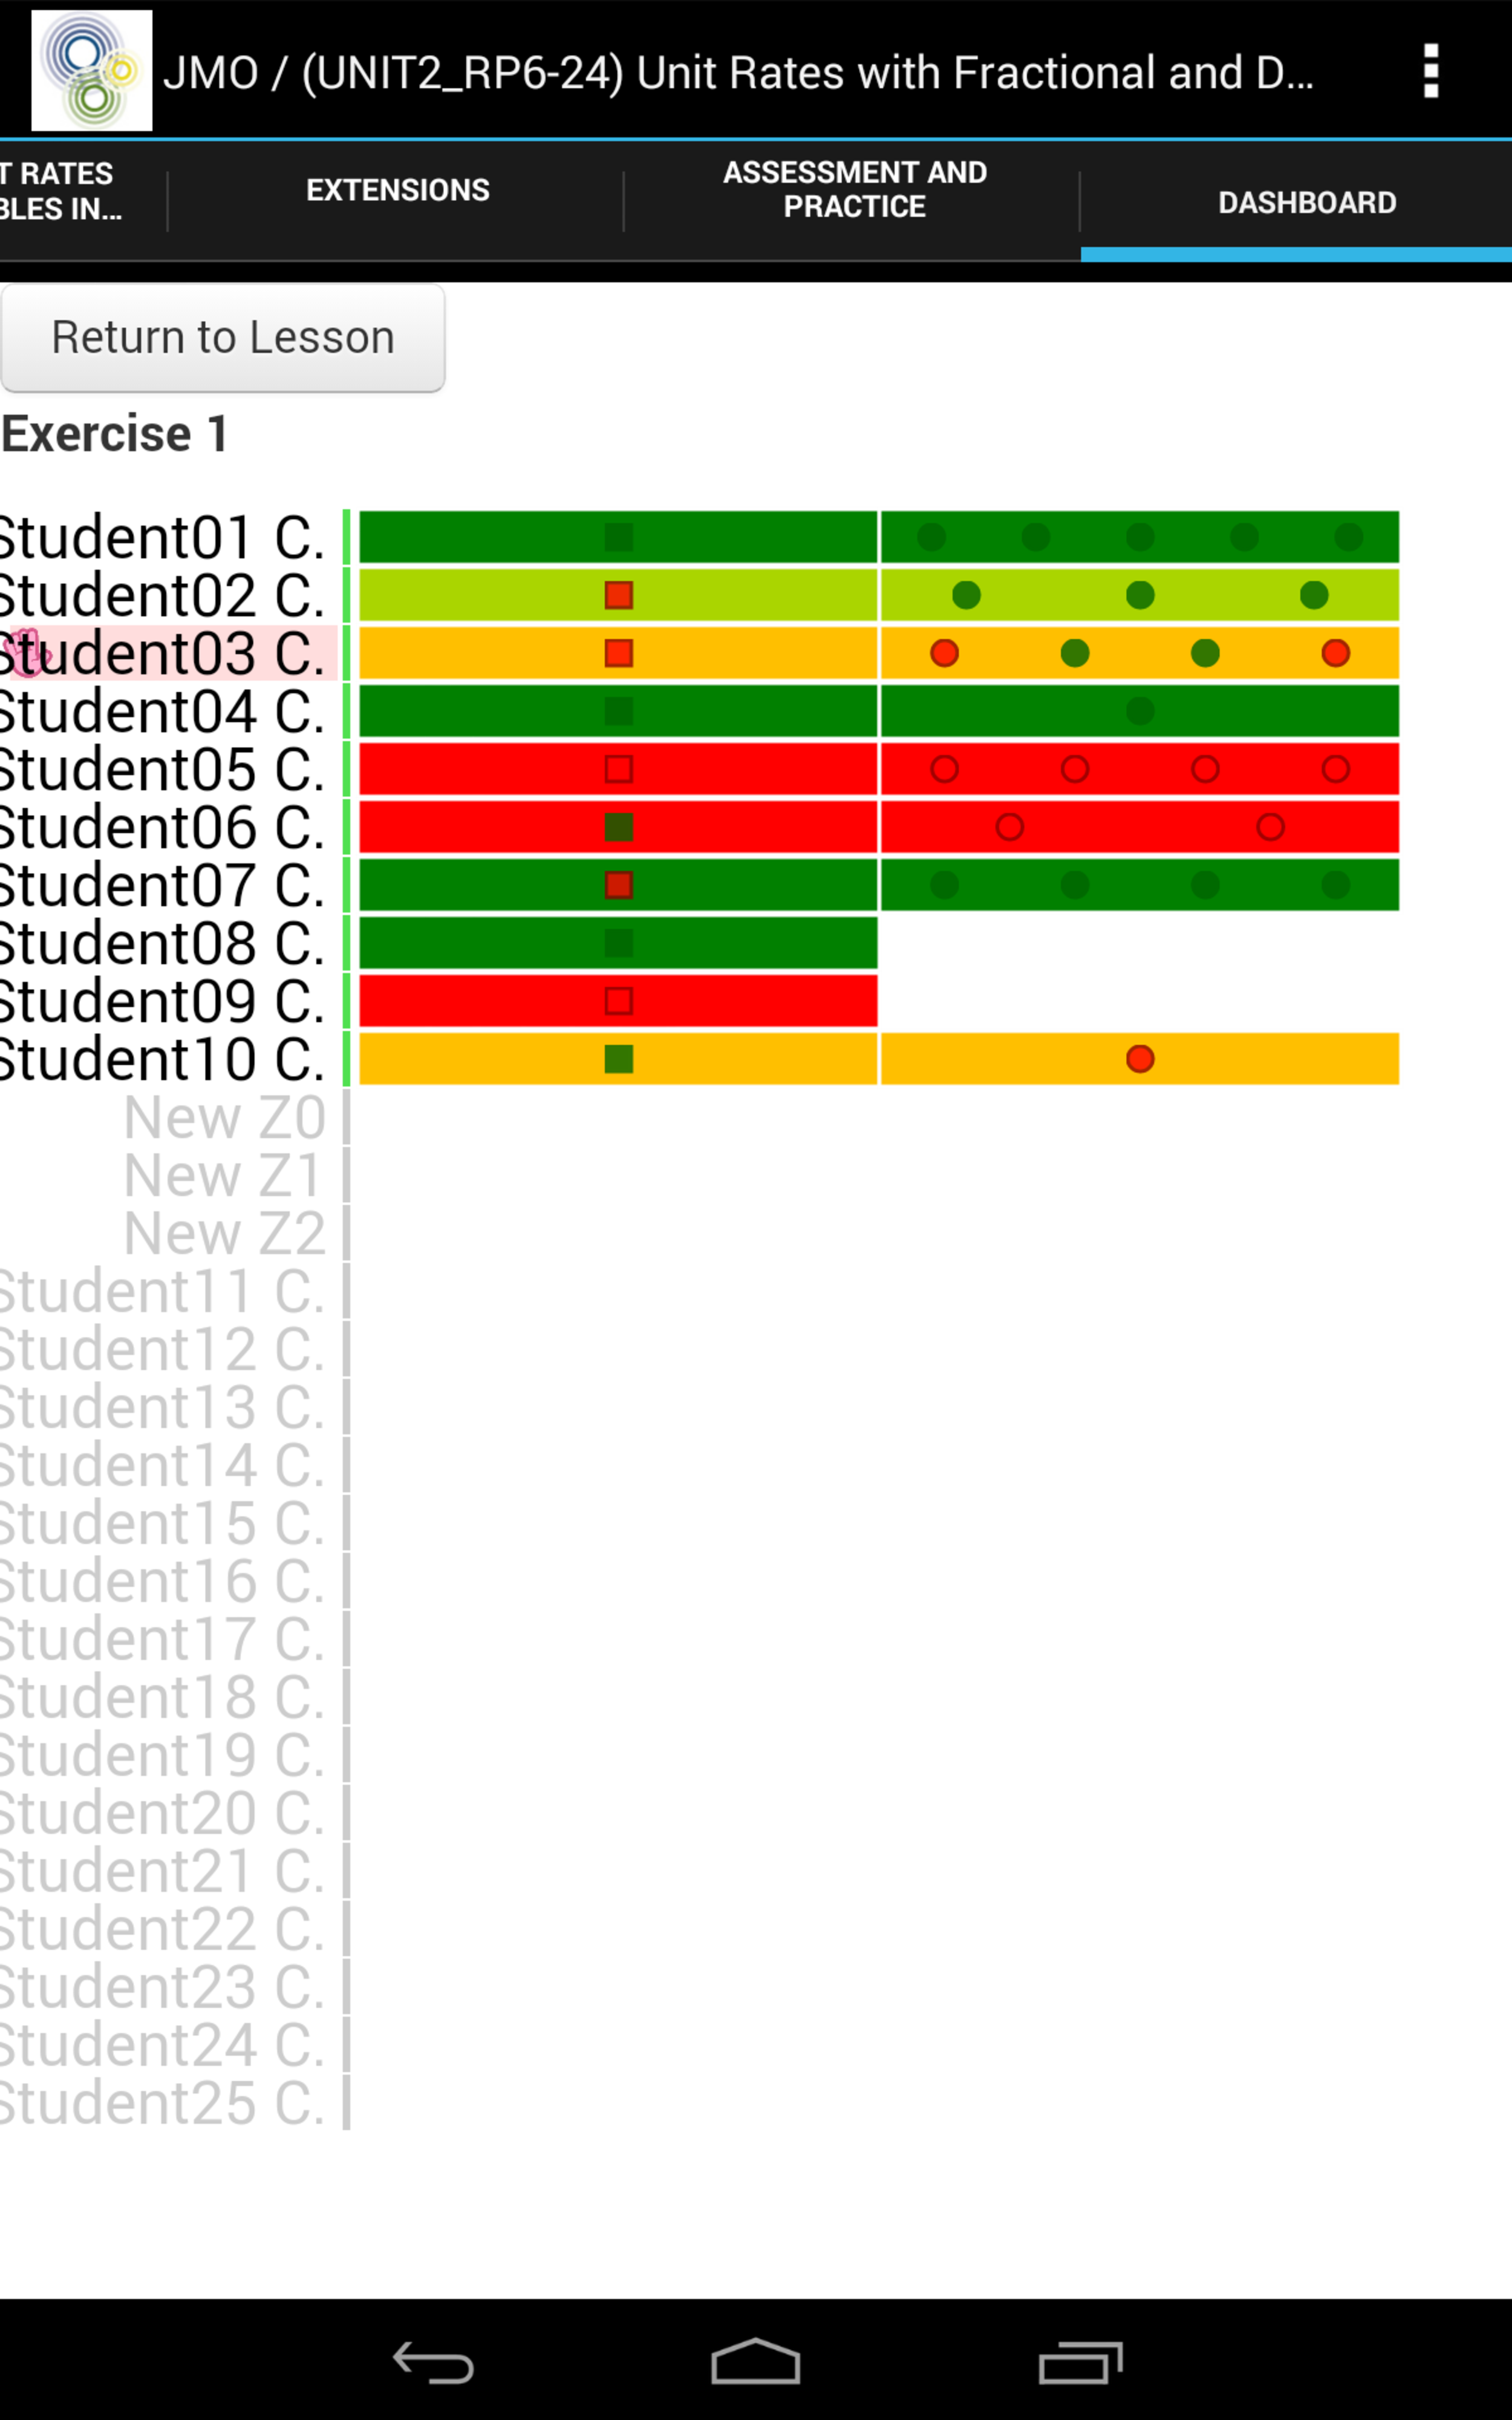
\includegraphics[width=40mm]{images/TeacherDashboard.pdf}} \hspace{1em}%
%\subfigure[]{\label{fig:StudentProblemSolving}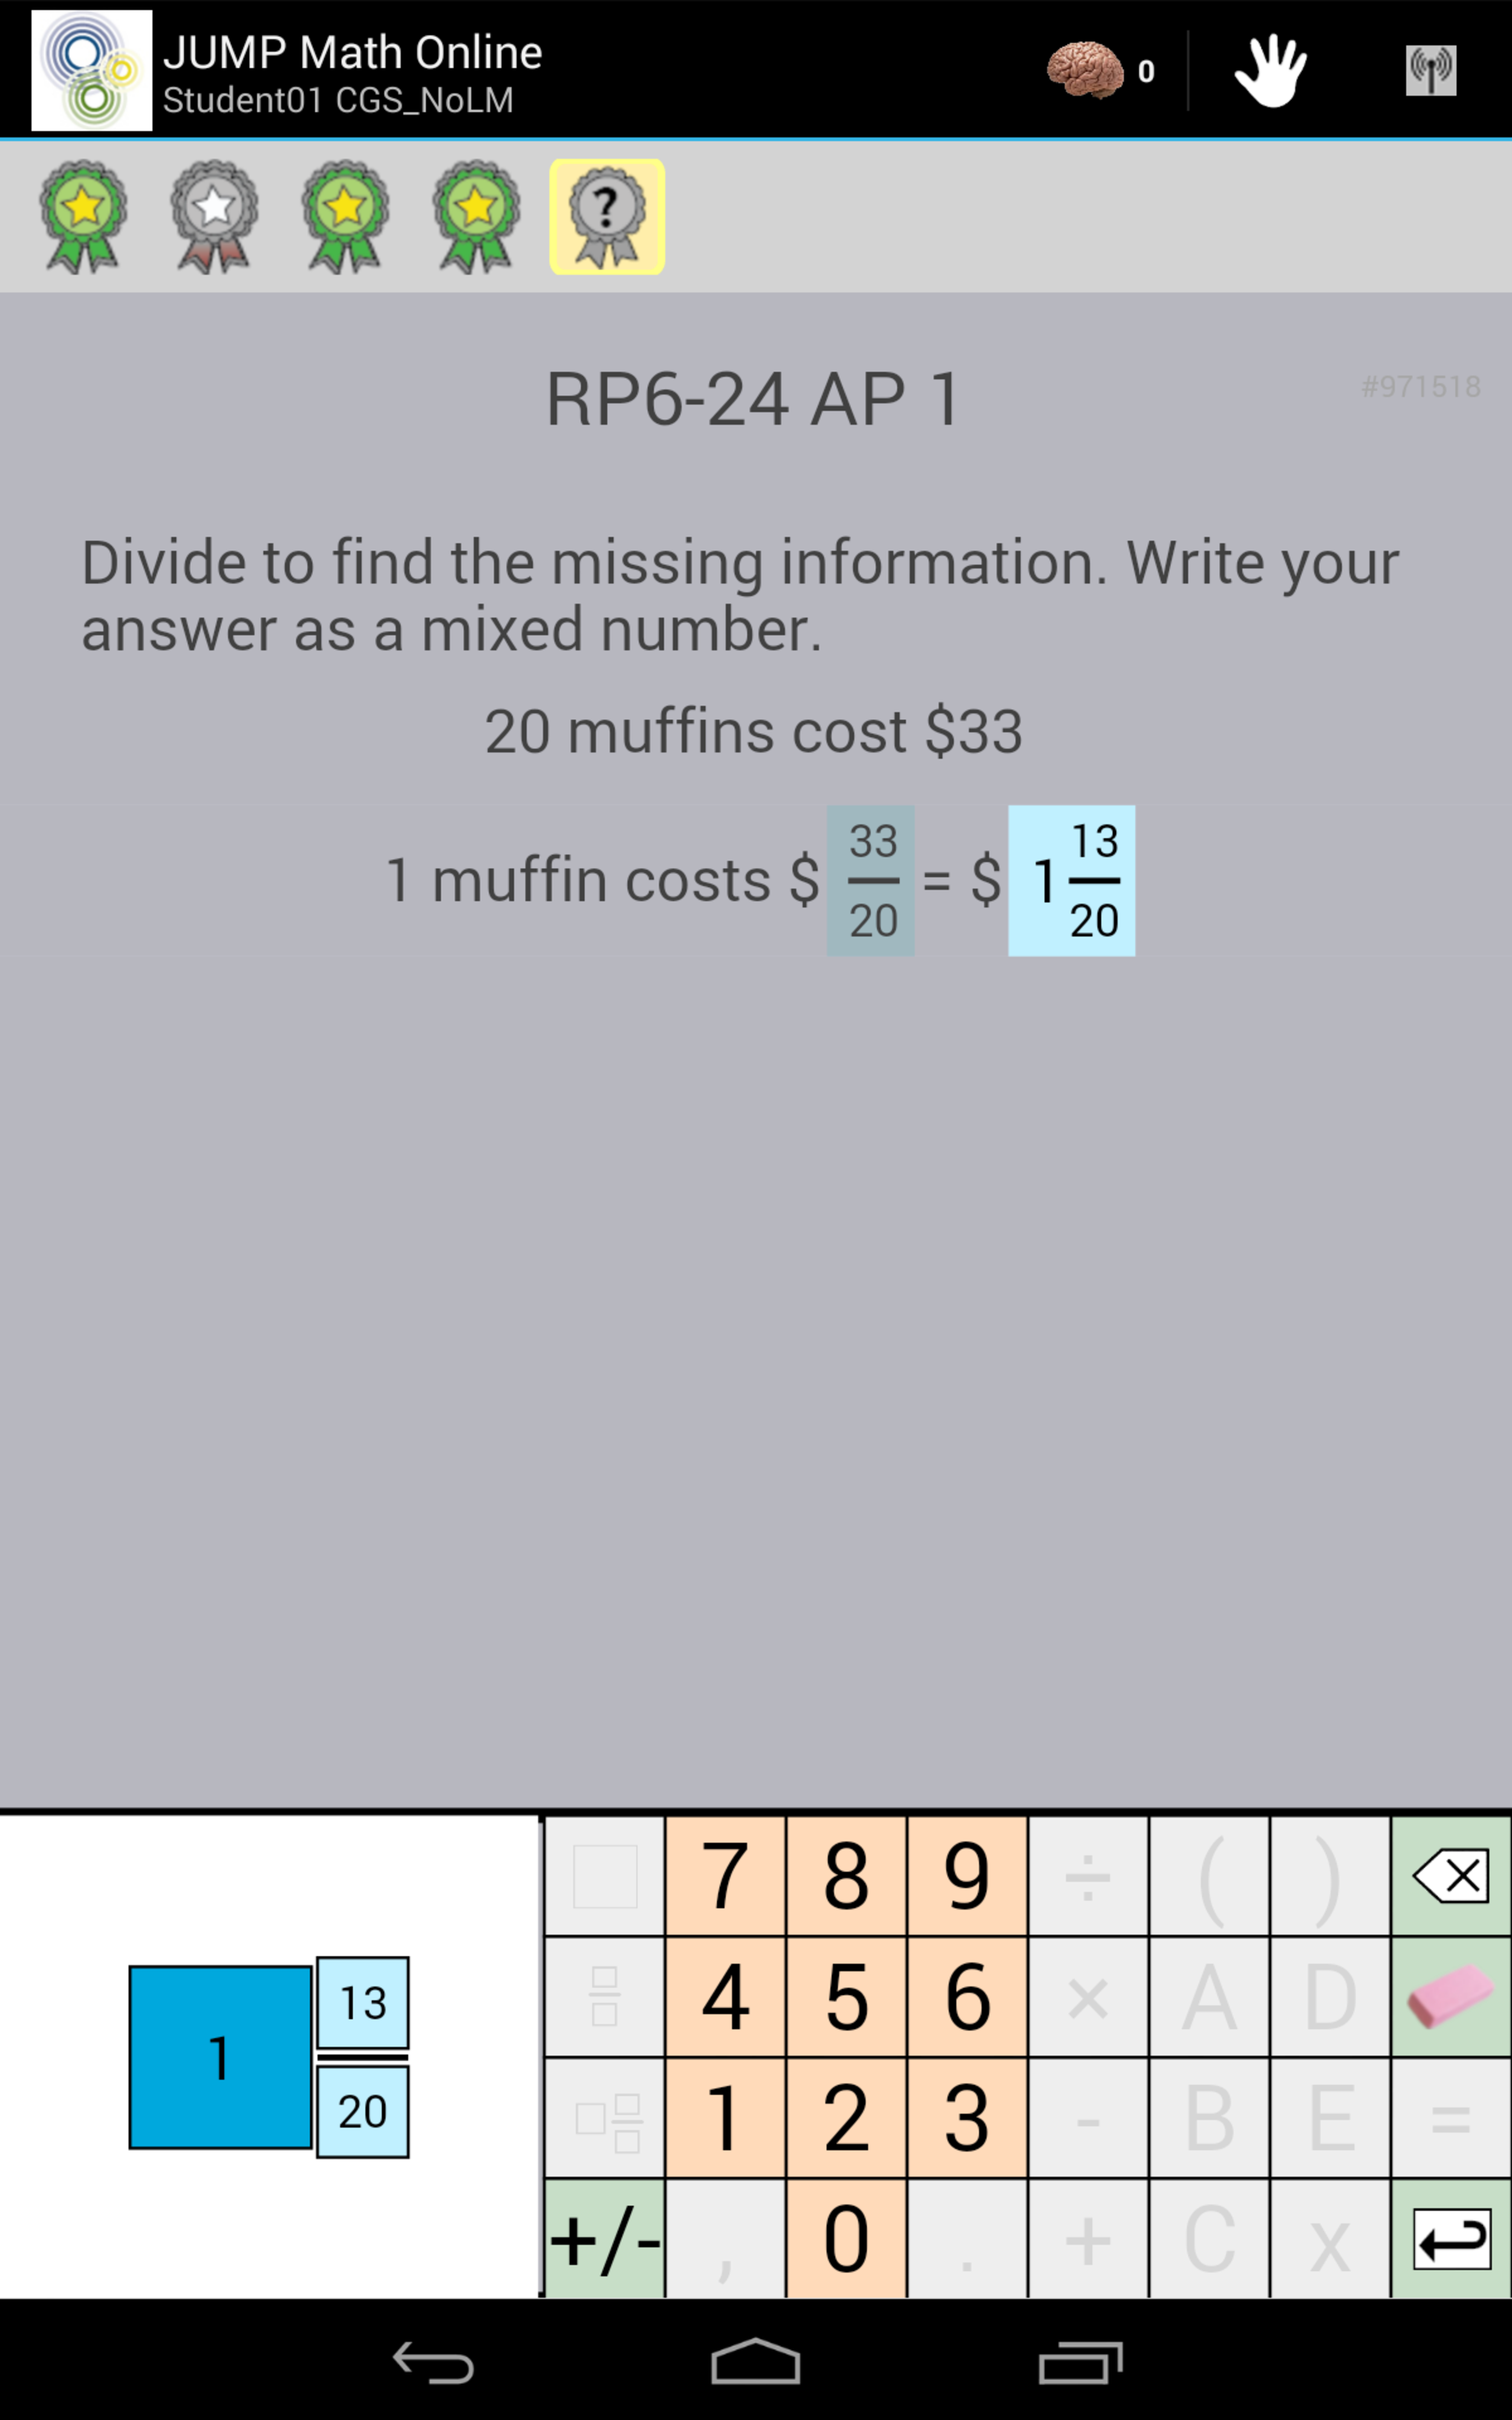
\includegraphics[width=40mm]{images/Student.pdf}}
%\caption{
%Screenshots of the Teacher and Student software. Figure (a) shows the teacher lesson view. Figure (b) shows a prompt for the teacher to ``Start Exercise 1'' on all student tablets. Figure (c) shows the teacher Dashboard that displays student problem-solving progress. Figure (d) shows the student problem-solving interface, with a calculator input interface at the bottom of the screen and badges at the top that indicate problem correctness. }
%\label{fig:Spreadsheet}
%\end{figure*}


% Balancing columns in a ref list is a bit of a pain because you
% either use a hack like flushend or balance, or manually insert
% a column break.  http://www.tex.ac.uk/cgi-bin/texfaq2html?label=balance
% multicols doesn't work because we're already in two-column mode,
% and flushend isn't awesome, so I choose balance.  See this
% for more info: http://cs.brown.edu/system/software/latex/doc/balance.pdf
%
% Note that in a perfect world balance wants to be in the first
% column of the last page.
%
% If balance doesn't work for you, you can remove that and
% hard-code a column break into the bbl file right before you
% submit:
%
% http://stackoverflow.com/questions/2149854/how-to-manually-equalize-columns-
% in-an-ieee-paper-if-using-bibtex
%
% Or, just remove \balance and give up on balancing the last page.
%
%\balance{}


% REFERENCES FORMAT
% References must be the same font size as other body text.
\bibliographystyle{SIGCHI-Reference-Format}
\small
\bibliography{references}

\end{document}

%%% Local Variables:
%%% mode: latex
%%% TeX-master: t
%%% End:
